% =====================================================================
%  Sparsity and Precision, Visually  --  lecture notes on the two levers
%  that cut the cost of an LLM: mixture of experts, pruning, activation
%  and attention sparsity; number formats, low-precision training,
%  precision scaling laws and quantization for inference.
%  Same visual language as "The Transformer, Visually".
%
%  Compile:  pdflatex sparsity_precision_tutorial.tex   (run twice)
%  Self-contained: every figure is TikZ/pgfplots source in this file.
%  Needs only standard packages: beamer, tikz/pgf, pgfplots, helvet,
%  amsmath, booktabs.
%
%  Conventions
%   * One color per component, used on every slide (see "palette").
%   * \stage{n} before a frame sets the accent color and highlights the
%     matching chip in the footer strip.
%   * Curves drawn from a paper's published constants are labelled with
%     the paper; curves labelled "illustrative" are sketches, not data.
% =====================================================================
\documentclass[aspectratio=169,11pt]{beamer}

% ---------- fonts ----------------------------------------------------
\usepackage[scaled=0.92]{helvet}        % Helvetica-like sans for text
\renewcommand{\ttdefault}{cmtt}         % Computer Modern mono for tokens
\usefonttheme[onlymath]{serif}          % classic serif math
\usepackage{amsmath,amssymb,bm}
\usepackage{booktabs,array}
\usepackage{graphicx}


% ---------- graphics -------------------------------------------------
\usepackage{tikz}
\usepackage{pgfplots}
\pgfplotsset{compat=1.17}
\usetikzlibrary{arrows.meta,positioning,calc,fit,backgrounds,
                decorations.pathreplacing,shapes.geometric}

% ---------- palette --------------------------------------------------
\definecolor{ink}{HTML}{1F2937}     % text, residual stream
\definecolor{muted}{HTML}{6B7280}   % secondary text
\definecolor{hair}{HTML}{D9DDE4}    % hairlines
\definecolor{paper}{HTML}{FCFCFA}   % slide background
\definecolor{tok}{HTML}{5F6F85}     % tokens / tokenizer
\definecolor{emb}{HTML}{0CA678}     % embeddings
\definecolor{posc}{HTML}{7048E8}     % positional information
\definecolor{attn}{HTML}{E8590C}    % attention
\definecolor{mlp}{HTML}{1C7ED6}     % MLP / feed-forward
\definecolor{norm}{HTML}{5C940D}    % normalization
\definecolor{outc}{HTML}{D6336C}     % unembedding / softmax / sampling
\definecolor{trn}{HTML}{9C6644}     % training and scaling
\colorlet{qc}{attn}                 % queries
\definecolor{kc}{HTML}{F59F00}      % keys
\definecolor{vc}{HTML}{1098AD}      % values
\colorlet{kct}{kc!70!black}         % key color, darkened for text
\colorlet{stagec}{ink}              % accent of the current stage

% ---------- beamer look ----------------------------------------------
\setbeamertemplate{navigation symbols}{}
\setbeamercolor{background canvas}{bg=paper}
\setbeamercolor{normal text}{fg=ink}
\setbeamercolor{frametitle}{fg=ink}
\setbeamersize{text margin left=8mm,text margin right=8mm}
\setbeamertemplate{itemize item}{\raisebox{0.25ex}{\tiny\color{stagec}$\blacksquare$}}
\setlength{\leftmargini}{1.1em}
\hyphenpenalty=10000 \exhyphenpenalty=10000   % no hyphenation on slides

% stage = which part of the pipeline the slide belongs to
\newcount\stageno \stageno=1
\newcommand{\stage}[1]{\global\stageno=#1\relax
  \ifcase#1\or\colorlet{stagec}{ink}\or\colorlet{stagec}{attn}%
  \or\colorlet{stagec}{tok}\or\colorlet{stagec}{emb}%
  \or\colorlet{stagec}{posc}\or\colorlet{stagec}{mlp}%
  \or\colorlet{stagec}{trn}\or\colorlet{stagec}{outc}%
  \or\colorlet{stagec}{vc}\or\colorlet{stagec}{ink}\fi}

\makeatletter
% title: accent bar + title + one-line claim (the frame subtitle)
\setbeamertemplate{frametitle}{%
  \nointerlineskip\vspace*{3.6mm}%
  \begin{tikzpicture}[x=1mm,y=1mm]
    \useasboundingbox (0,0) rectangle (144,10.5);
    \fill[stagec,rounded corners=0.5mm] (0,0.3) rectangle (1.5,10.2);
    \ifx\insertframesubtitle\@empty
      \node[anchor=west,inner sep=0,text=ink,
            font=\fontsize{15}{17}\selectfont\bfseries] at (4.2,5.2) {\insertframetitle};
    \else
      \node[anchor=west,inner sep=0,text=ink,
            font=\fontsize{15}{17}\selectfont\bfseries] at (4.2,7.1) {\insertframetitle};
      \node[anchor=west,inner sep=0,text=muted,
            font=\fontsize{8.6}{10}\selectfont] at (4.2,2.0) {\insertframesubtitle};
    \fi
  \end{tikzpicture}}
\makeatother

% footer: pipeline strip with the current stage lit, plus page number
\setbeamertemplate{footline}{%
  
\begin{tikzpicture}[x=1mm,y=1mm]
    \useasboundingbox (0,0) rectangle (160,7.2);
    \coordinate (c0) at (7.2,4.0);
    \foreach \lab/\col [count=\i,remember=\i as \prev (initially 0)] in
      {Overview/ink,MoE/attn,Pruning/tok,Activations/emb,Formats/posc,
       Training/mlp,Laws/trn,Quantization/outc,Practice/vc,Wrap-up/ink}{
      \ifnum\i=\stageno
        \node[anchor=west,inner xsep=1.5mm,inner ysep=0.75mm,rounded corners=0.7mm,
              fill=\col,text=white,text height=1.5ex,text depth=0.35ex,
              font=\fontsize{5.8}{7}\selectfont\bfseries] (c\i) at ([xshift=0.8mm]c\prev.east) {\lab};
      \else
        \node[anchor=west,inner xsep=1.5mm,inner ysep=0.75mm,
              text=muted!80,text height=1.5ex,text depth=0.35ex,
              font=\fontsize{5.8}{7}\selectfont] (c\i) at ([xshift=0.8mm]c\prev.east) {\lab};
      \fi}
    \node[anchor=east,inner sep=0,text=muted,
          font=\fontsize{6.5}{8}\selectfont] at (152,4.0)
          {\insertframenumber\,/\,\inserttotalframenumber};
  \end{tikzpicture}}

% ---------- TikZ vocabulary ------------------------------------------
\tikzset{
  >={Stealth[length=4.6pt,width=4pt]},
  flow/.style={->,line width=0.8pt,draw=ink!70},
  thinflow/.style={->,line width=0.5pt,draw=ink!55},
  % component box (tinted) and its solid variant; argument = color
  comp/.style={rounded corners=2.2pt,draw=#1,fill=#1!12,line width=0.8pt,
               align=center,inner sep=4pt,font=\small,text=ink},
  fillbox/.style={rounded corners=2.2pt,fill=#1,text=white,align=center,
                inner sep=4pt,font=\small\bfseries},
  % a token
  chip/.style={rounded corners=1.8pt,fill=tok!14,draw=tok!55,line width=0.5pt,
               font=\ttfamily\footnotesize,inner xsep=3.5pt,inner ysep=2.5pt,
               text height=1.5ex,text depth=0.45ex,text=ink},
  cchip/.style={chip,fill=#1!16,draw=#1!75},
  lab/.style={font=\scriptsize,text=muted,inner sep=1.5pt},
  txt/.style={font=\footnotesize,text=ink,align=flush left,inner sep=0pt},
  plus/.style={circle,draw=ink,fill=paper,line width=0.75pt,inner sep=0pt,
               minimum size=9.5pt,font=\scriptsize\bfseries},
  brace/.style={decorate,decoration={brace,amplitude=3.5pt},draw=muted,line width=0.6pt},
}

% \cells{x}{y}{size}{color}{shade,shade,...}: a row of vector cells
\newcommand{\cells}[5]{%
  \foreach \sh [count=\ci from 0] in {#5}{%
    \fill[#4!\sh!white,draw=paper,line width=0.4pt]
      ({#1+\ci*#3},{#2}) rectangle ++(#3,#3);}}

% \rgrid{x}{y}{rows}{cols}{size}{color}{seed}: a matrix with varied shading
\newcommand{\rgrid}[7]{%
  \foreach \ri in {1,...,#3}{\foreach \ci in {1,...,#4}{%
    \pgfmathtruncatemacro\sh{16+mod(\ri*37+\ci*53+\ri*\ci*11+#7*29,8)*10}%
    \fill[#6!\sh!white,draw=paper,line width=0.4pt]
      ({#1+(\ci-1)*#5},{#2+(#3-\ri)*#5}) rectangle ++(#5,#5);}}}

% \barh{x}{y}{length}{color}: one horizontal bar of a bar chart
\newcommand{\barh}[4]{\fill[#4,rounded corners=0.8pt] ({#1},{#2-0.13}) rectangle ++({#3},0.26);}

% \valgrid{x}{y}{size}{color}{scale}{mask}{\rows}: matrix shaded by value.
% (x,y) is the top-left corner; \rows is a macro holding {a,b,..},{..},..
% With mask=1 the cells above the diagonal are drawn as blocked.
\newcommand{\valgrid}[7]{%
  \edef\vglist{#7}%
  \foreach \row [count=\r from 0] in \vglist {\foreach \v [count=\c from 0] in \row {%
    \pgfmathtruncatemacro\sh{min(100,\v*#5)}%
    \pgfmathtruncatemacro\msk{and(#6>0,\c>\r)}%
    \ifnum\msk=1
      \fill[tok!10,draw=paper,line width=0.4pt] ({#1+\c*#3},{#2-(\r+1)*#3}) rectangle ++(#3,#3);
    \else
      \fill[#4!\sh!white,draw=paper,line width=0.4pt] ({#1+\c*#3},{#2-(\r+1)*#3}) rectangle ++(#3,#3);
    \fi}}}

% the running attention example: Alice thanked Bob because she
\def\Sraw{{2.0,0.7,1.3,0.4,1.1},{1.8,1.2,0.9,1.6,0.5},{0.6,1.5,1.9,0.8,1.4},
          {0.8,1.6,0.9,1.1,2.1},{3.1,0.9,1.4,1.0,1.5}}          % scores
\def\Aw{{1.00,0,0,0,0},{.65,.35,0,0,0},{.14,.35,.51,0,0},
        {.18,.39,.19,.24,0},{.62,.07,.11,.08,.12}}              % softmax rows

% paper figure: \paperfig{file}{width}{Figure n}
\newcommand{\paperfig}[3]{%
  \begin{tikzpicture}
    \node[inner sep=0] (img) {\includegraphics[width=#2]{#1}};
    \node[anchor=north east,font=\fontsize{5.5}{6}\selectfont,text=muted,
          rounded corners=1pt,fill=ink!6,inner sep=2pt] at ([xshift=-1mm,yshift=-1mm]img.north east) {report, #3};
  \end{tikzpicture}}
% background panel: \bgpanel{x}{y}{width}{title}{body}  (anchor north west)
\newcommand{\bgpanel}[5]{%
  \node[anchor=north west,inner sep=0] at (#1,#2) {%
    \begin{tikzpicture}
      \node[anchor=north west,text width=#3,align=flush left,font=\footnotesize,text=ink,
            inner xsep=8pt,inner ysep=6pt,rounded corners=3pt,fill=stagec!7] (bp)
            {{\color{stagec}\bfseries\scriptsize #4}\\[3pt]#5};
      \fill[stagec,rounded corners=1.5pt] (bp.north west) rectangle ([xshift=3pt]bp.south west);
    \end{tikzpicture}};}
% same panel with a smaller body font, for denser slides
\newcommand{\bgpanels}[5]{%
  \node[anchor=north west,inner sep=0] at (#1,#2) {%
    \begin{tikzpicture}
      \node[anchor=north west,text width=#3,align=flush left,font=\scriptsize,text=ink,
            inner xsep=8pt,inner ysep=6pt,rounded corners=3pt,fill=stagec!7] (bp)
            {{\color{stagec}\bfseries\scriptsize #4}\\[3pt]#5};
      \fill[stagec,rounded corners=1.5pt] (bp.north west) rectangle ([xshift=3pt]bp.south west);
    \end{tikzpicture}};}
% stat tile: \stat{x}{y}{value}{label}{color}
\newcommand{\stat}[5]{%
  \node[anchor=north west,inner sep=0] at (#1,#2) {%
    \begin{tikzpicture}
      \node[anchor=north west,minimum width=3.2cm,minimum height=1.45cm,rounded corners=3pt,
            fill=#5!10,draw=#5!50,line width=0.6pt] (t) {};
      \node[anchor=north west,font=\fontsize{15}{16}\selectfont\bfseries,text=#5!85!black,inner sep=0]
            at ([xshift=7pt,yshift=-7pt]t.north west) {#3};
      \node[anchor=south west,font=\scriptsize,text=ink,inner sep=0,text width=2.9cm,align=left]
            at ([xshift=7pt,yshift=6pt]t.south west) {#4};
    \end{tikzpicture}};}

% small source tag inside a figure: \srctag{x}{y}{text}
\newcommand{\srctag}[3]{\node[anchor=north east,font=\fontsize{5.5}{6}\selectfont,text=muted,
  rounded corners=1pt,fill=ink!6,inner sep=2pt] at (#1,#2) {#3};}
% axis style shared by all plots
\pgfplotsset{lecture/.style={axis lines=left,axis line style={muted,line width=0.5pt},
  tick style={muted},tick label style={font=\scriptsize,text=muted},
  label style={font=\scriptsize,text=muted},grid=major,grid style={hair,line width=0.4pt},
  legend style={draw=none,fill=none,font=\scriptsize,legend cell align=left,row sep=1pt},
  clip=false}}

% chat message: \msg{x}{y}{width}{role color}{role}{text}  (anchor north west)
\newcommand{\msg}[6]{%
  \node[anchor=north west,inner sep=0] at (#1,#2) {%
    \begin{tikzpicture}
      \node[anchor=north west,text width=#3,align=flush left,font=\scriptsize,text=ink,
            inner xsep=5pt,inner ysep=4pt,rounded corners=3pt,fill=#4!8,draw=#4!35,line width=0.4pt] (m) {#6};
      \node[anchor=south west,font=\tiny\bfseries,text=#4,inner sep=1pt] at ([yshift=0.5pt]m.north west) {#5};
    \end{tikzpicture}};}
% pipeline chevron: \chev{x}{y}{width}{color}{label}
\newcommand{\chev}[5]{%
  \fill[#4,rounded corners=1pt] (#1,#2) -- ({#1+#3-0.22},#2) -- ({#1+#3},{#2+0.3}) -- ({#1+#3-0.22},{#2+0.6}) -- (#1,{#2+0.6}) -- ({#1+0.22},{#2+0.3}) -- cycle;
  \node[text=white,font=\scriptsize\bfseries] at ({#1+#3/2},{#2+0.3}) {#5};}

% short text helpers
\newcommand{\hl}[2]{{\color{#1}\bfseries #2}}
\newcommand{\tokt}[1]{{\ttfamily #1}}

\begin{document}

% ---------------------------------------------------------------- 1
{\setbeamertemplate{footline}{}
\begin{frame}[plain]

\begin{tikzpicture}[remember picture,overlay,x=1mm,y=1mm,
                    shift={(current page.south west)}]
  % cover graphic: a weight matrix, half the entries pruned, the rest in four shades
  \begin{scope}[shift={(104,14)}]
    \foreach \r in {0,...,8}{\foreach \c in {0,...,9}{
      \pgfmathtruncatemacro{\keep}{mod(\r*37+\c*53+\r*\c*11,7)<4}
      \pgfmathtruncatemacro{\sh}{25+mod(\r*17+\c*29,4)*25}
      \ifnum\keep=1
        \fill[attn!\sh!white,rounded corners=0.3mm] (\c*4.6,\r*4.6) rectangle ++(4.0,4.0);
      \else
        \draw[hair,line width=0.3pt,rounded corners=0.3mm] (\c*4.6,\r*4.6) rectangle ++(4.0,4.0);
      \fi}}
    \node[font=\fontsize{5.5}{6}\selectfont,text=muted,anchor=north west] at (0,-1.5) {blank: pruned \quad four shades: 2-bit values};
  \end{scope}
  \fill[attn] (12,60.5) rectangle (26,61.6);
  \node[anchor=south west,inner sep=0,text=muted,
        font=\fontsize{10}{12}\selectfont\bfseries] at (12,63.5) {LECTURE NOTES \ $\cdot$ \ EFFICIENCY, 2026};
  \node[anchor=south west,inner sep=0,text=ink,align=left,
        font=\fontsize{30}{34}\selectfont\bfseries] at (12,38)
        {Sparsity and\\Precision, Visually};
  \node[anchor=north west,inner sep=0,text=muted,align=flush left,text width=76mm,
        font=\fontsize{11}{15}\selectfont] at (12,33)
        {The two levers that cut the cost of a language model: mixture of
         experts, pruning, sparse activations and sparse attention; number
         formats, low-precision training, precision scaling laws, and
         quantization for inference.};
\end{tikzpicture}
\end{frame}}

% ---------------------------------------------------------------- 2
\stage{1}
\begin{frame}{Two levers on one cost model}
\framesubtitle{Sparsity cuts how many numbers each token touches; precision cuts how many bits each number has.}
\centering
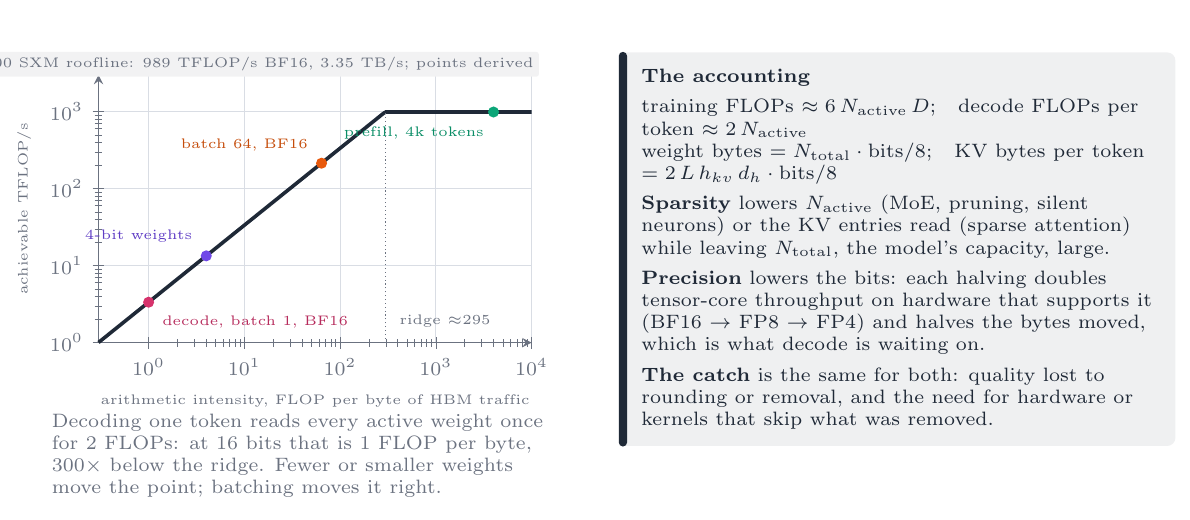
\begin{tikzpicture}
  \useasboundingbox (0,0) rectangle (14.4,5.9);
  \begin{axis}[lecture,at={(0.9cm,1.9cm)},anchor=south west,scale only axis,width=5.5cm,height=3.4cm,
      xmode=log,ymode=log,xmin=0.3,xmax=10000,ymin=1,ymax=3000,domain=0.3:10000,samples=200,
      xtick={1,10,100,1000,10000},ytick={1,10,100,1000},
      xlabel={arithmetic intensity, FLOP per byte of HBM traffic},ylabel={achievable TFLOP/s},
      x label style={font=\tiny},y label style={font=\tiny}]
    \addplot[ink,line width=1.3pt] {min(3.35*x,989)};
    \draw[muted,densely dotted] (axis cs:295,1) -- (axis cs:295,989);
    \node[font=\tiny,text=muted,anchor=south west] at (axis cs:330,1.2) {ridge $\approx$295};
    \fill[outc] (axis cs:1,3.35) circle (2pt); \node[font=\tiny,text=outc!85!black,anchor=north west] at (axis cs:1.1,3.0) {decode, batch 1, BF16};
    \fill[posc] (axis cs:4,13.4) circle (2pt); \node[font=\tiny,text=posc!85!black,anchor=south east] at (axis cs:3.6,15) {4-bit weights};
    \fill[attn] (axis cs:64,214) circle (2pt); \node[font=\tiny,text=attn!85!black,anchor=south east] at (axis cs:58,230) {batch 64, BF16};
    \fill[emb] (axis cs:4000,989) circle (2pt); \node[font=\tiny,text=emb!85!black,anchor=north east] at (axis cs:4000,850) {prefill, 4k tokens};
  \end{axis}
  \srctag{6.5}{5.6}{H100 SXM roofline: 989 TFLOP/s BF16, 3.35 TB/s; points derived}
  \node[txt,anchor=north west,text width=6.3cm,font=\scriptsize,text=muted] at (0.3,1.0)
    {Decoding one token reads every active weight once for 2 FLOPs: at 16 bits that is 1 FLOP per byte, 300$\times$ below the ridge. Fewer or smaller weights move the point; batching moves it right.};
  \bgpanels{7.5}{5.6}{6.5cm}{The accounting}{%
    training FLOPs $\approx 6\,N_{\text{active}}\,D$;\quad decode FLOPs per token $\approx 2\,N_{\text{active}}$\\
    weight bytes $= N_{\text{total}}\cdot\text{bits}/8$;\quad KV bytes per token $=2\,L\,h_{kv}\,d_h\cdot\text{bits}/8$\\[3pt]
    \hl{ink}{Sparsity} lowers $N_{\text{active}}$ (MoE, pruning, silent neurons)
    or the KV entries read (sparse attention) while leaving $N_{\text{total}}$,
    the model's capacity, large.\\[3pt]
    \hl{ink}{Precision} lowers the bits: each halving doubles tensor-core
    throughput on hardware that supports it (BF16 $\to$ FP8 $\to$ FP4) and
    halves the bytes moved, which is what decode is waiting on.\\[3pt]
    \hl{ink}{The catch} is the same for both: quality lost to rounding or
    removal, and the need for hardware or kernels that skip what was
    removed.}
\end{tikzpicture}
\end{frame}

% ---------------------------------------------------------------- 3
\begin{frame}{The map, and a timeline}
\framesubtitle{Four kinds of sparsity, four questions about precision, and when each arrived in language models.}
\centering
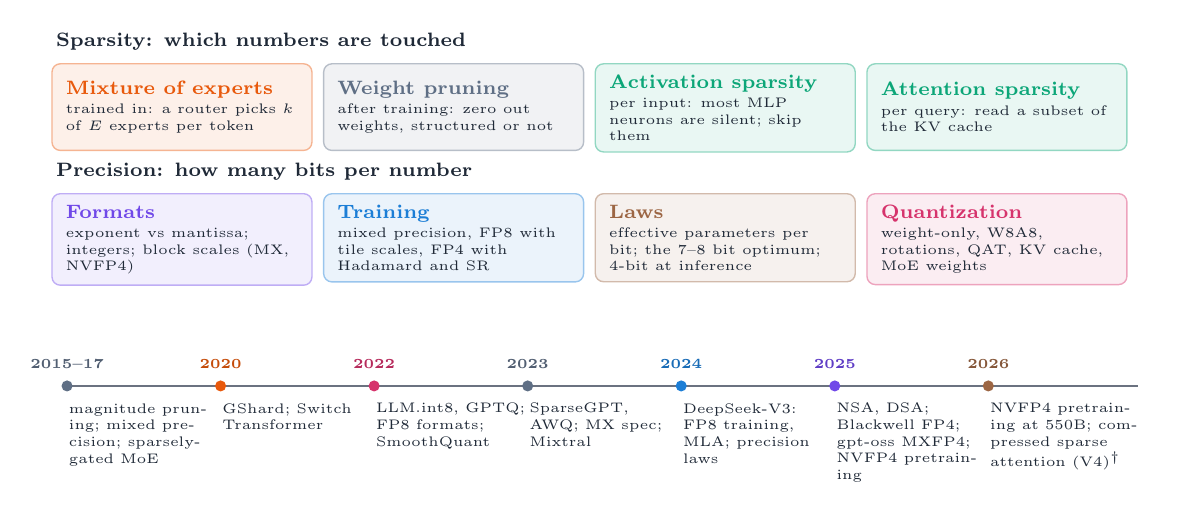
\begin{tikzpicture}
  \useasboundingbox (0,0) rectangle (14.4,5.9);
  \node[lab,anchor=south west,font=\scriptsize\bfseries,text=ink] at (0.3,5.55) {Sparsity: which numbers are touched};
  \foreach \i/\c/\ttl/\body in {0/attn/{Mixture of experts}/{trained in: a router picks $k$ of $E$ experts per token},
                                1/tok/{Weight pruning}/{after training: zero out weights, structured or not},
                                2/emb/{Activation sparsity}/{per input: most MLP neurons are silent; skip them},
                                3/emb/{Attention sparsity}/{per query: read a subset of the KV cache}}{
    \node[anchor=north west,text width=2.95cm,align=flush left,font=\tiny,text=ink,minimum height=1.1cm,
          inner xsep=5pt,inner ysep=4pt,rounded corners=3pt,fill=\c!9,draw=\c!45,line width=0.5pt] at ({0.3+\i*3.45},5.45)
          {{\color{\c}\bfseries\scriptsize\ttl}\\[1pt]\body};}
  \node[lab,anchor=south west,font=\scriptsize\bfseries,text=ink] at (0.3,3.9) {Precision: how many bits per number};
  \foreach \i/\c/\ttl/\body in {0/posc/{Formats}/{exponent vs mantissa; integers; block scales (MX, NVFP4)},
                                1/mlp/{Training}/{mixed precision, FP8 with tile scales, FP4 with Hadamard and SR},
                                2/trn/{Laws}/{effective parameters per bit; the 7--8 bit optimum; 4-bit at inference},
                                3/outc/{Quantization}/{weight-only, W8A8, rotations, QAT, KV cache, MoE weights}}{
    \node[anchor=north west,text width=2.95cm,align=flush left,font=\tiny,text=ink,minimum height=1.1cm,
          inner xsep=5pt,inner ysep=4pt,rounded corners=3pt,fill=\c!9,draw=\c!45,line width=0.5pt] at ({0.3+\i*3.45},3.8)
          {{\color{\c}\bfseries\scriptsize\ttl}\\[1pt]\body};}
  % timeline
  \draw[muted,line width=0.6pt] (0.5,1.35) -- (14.1,1.35);
  \foreach \x/\yr/\t/\c in {0.5/{2015--17}/{magnitude pruning; mixed precision; sparsely-gated MoE}/tok,
                            2.45/2020/{GShard; Switch Transformer}/attn,4.4/2022/{LLM.int8, GPTQ; FP8 formats; SmoothQuant}/outc,
                            6.35/2023/{SparseGPT, AWQ; MX spec; Mixtral}/tok,8.3/2024/{DeepSeek-V3: FP8 training, MLA; precision laws}/mlp,
                            10.25/2025/{NSA, DSA; Blackwell FP4; gpt-oss MXFP4; NVFP4 pretraining}/posc,12.2/2026/{NVFP4 pretraining at 550B; compressed sparse attention (V4)$^\dagger$}/trn}{
    \fill[\c] (\x,1.35) circle (2pt);
    \node[font=\tiny\bfseries,text=\c!85!black,anchor=south] at (\x,1.45) {\yr};
    \node[font=\tiny,text=ink,anchor=north west,text width=1.9cm,align=left] at (\x-0.1,1.25) {\t};}
\end{tikzpicture}
\end{frame}

% ---------------------------------------------------------------- 4
\stage{2}
\begin{frame}{The mixture-of-experts layer}
\framesubtitle{Replace one wide MLP by $E$ narrow ones and a router; each token uses $k$ of them, so FLOPs follow $k$, not $E$.}
\centering
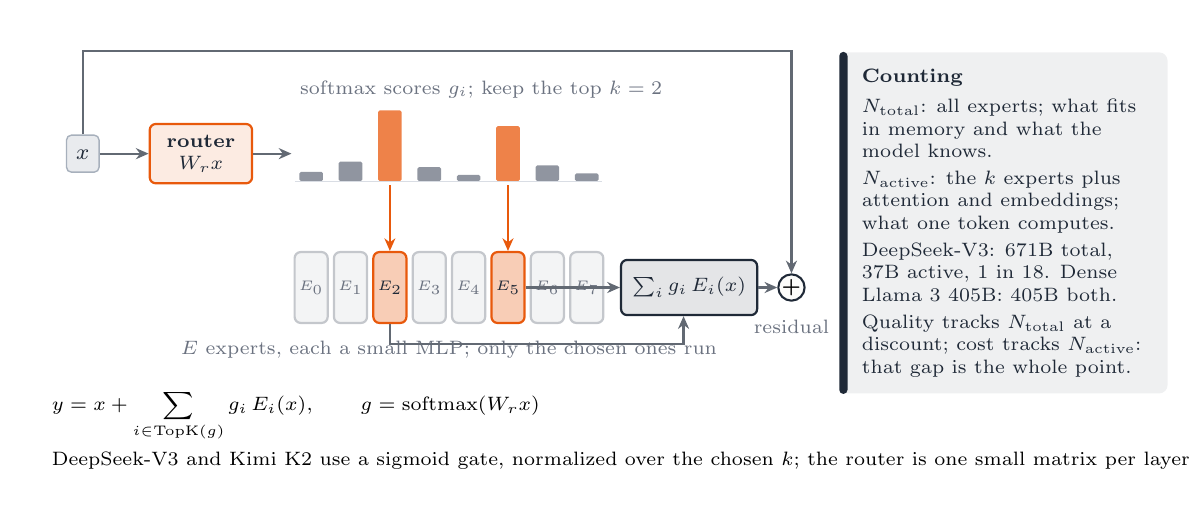
\begin{tikzpicture}
  \useasboundingbox (0,0) rectangle (14.4,5.9);
  \node[chip,fill=tok!14,draw=tok!55] (x) at (0.7,4.3) {$x$};
  \node[comp=attn,minimum width=1.3cm,minimum height=0.7cm,font=\scriptsize\bfseries,align=center] (rt) at (2.2,4.3) {router\\$W_r x$};
  \draw[flow] (x) -- (rt);
  % gate bars
  \foreach \i/\h/\c in {0/0.12/muted,1/0.25/muted,2/0.9/attn,3/0.18/muted,4/0.08/muted,5/0.7/attn,6/0.2/muted,7/0.1/muted}{
    \fill[\c!75,rounded corners=0.6pt] ({3.45+\i*0.5},3.95) rectangle ++(0.3,\h);}
  \draw[hair,line width=0.4pt] (3.4,3.95) -- (7.3,3.95);
  \node[lab,anchor=south west] at (3.4,4.95) {softmax scores $g_i$; keep the top $k=2$};
  \draw[flow] (rt.east) -- (3.35,4.3);
  % experts
  \foreach \i in {0,...,7}{
    \pgfmathtruncatemacro{\act}{ifthenelse(\i==2||\i==5,1,0)}
    \ifnum\act=1
      \node[comp=attn,fill=attn!30,minimum width=0.42cm,minimum height=0.9cm,inner xsep=1pt,font=\tiny\bfseries] (e\i) at ({3.6+\i*0.5},2.6) {$E_{\i}$};
      \draw[thinflow,attn] ({3.6+\i*0.5},3.9) -- (e\i.north);
    \else
      \node[comp=muted,fill=muted!8,draw=muted!40,minimum width=0.42cm,minimum height=0.9cm,inner xsep=1pt,font=\tiny,text=muted] (e\i) at ({3.6+\i*0.5},2.6) {$E_{\i}$};
    \fi}
  \node[lab,anchor=north,text width=7.4cm,align=center] at (5.35,1.98) {$E$ experts, each a small MLP; only the chosen ones run};
  \node[comp=ink,minimum width=1.5cm,minimum height=0.7cm,font=\scriptsize,align=center] (sum) at (8.4,2.6) {$\sum_i g_i\,E_i(x)$};
  \draw[flow] (e2.south) -- ++(0,-0.25) -| ([xshift=-2pt]sum.south);
  \draw[flow] (e5.east) -- (sum.west);
  \node[plus] (pl) at (9.7,2.6) {+};
  \draw[flow] (sum) -- (pl);
  \draw[flow] (x.north) -- (0.7,5.6) -| (pl.north);
  \node[lab,anchor=north] at (9.7,2.25) {residual};
  \node[anchor=north west,inner sep=0,font=\scriptsize,align=left] at (0.3,1.3)
    {$y=x+\displaystyle\sum_{i\in\mathrm{TopK}(g)} g_i\,E_i(x),\qquad g=\mathrm{softmax}(W_r x)$\\[3pt]
     DeepSeek-V3 and Kimi K2 use a sigmoid gate, normalized over the chosen $k$; the router is one small matrix per layer.};
  \bgpanels{10.3}{5.6}{3.6cm}{Counting}{%
    $N_{\text{total}}$: all experts; what fits in memory and what the model
    knows.\\[2pt]
    $N_{\text{active}}$: the $k$ experts plus attention and embeddings; what
    one token computes.\\[2pt]
    DeepSeek-V3: 671B total, 37B active, 1 in 18. Dense Llama 3 405B:
    405B both.\\[2pt]
    Quality tracks $N_{\text{total}}$ at a discount; cost tracks
    $N_{\text{active}}$: that gap is the whole point.}
\end{tikzpicture}
\end{frame}

% ---------------------------------------------------------------- 5
\begin{frame}{Routing: keeping the experts busy, and fed}
\framesubtitle{Left alone, a router sends most tokens to a few experts. Every recipe adds a pressure toward balance.}
\centering
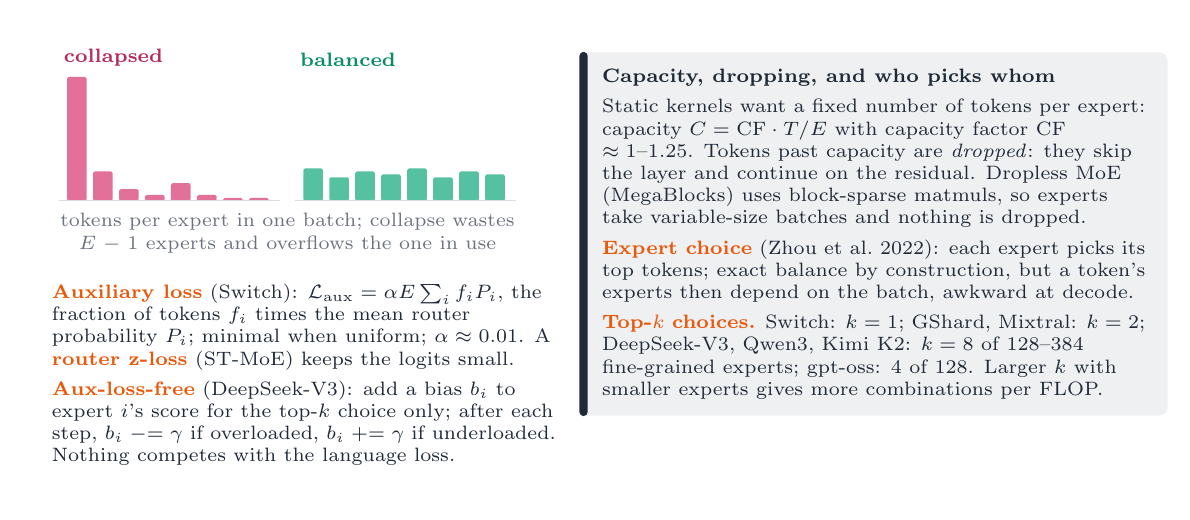
\begin{tikzpicture}
  \useasboundingbox (0,0) rectangle (14.4,5.9);
  % two load histograms
  \foreach \i/\h in {0/2.1,1/0.5,2/0.2,3/0.1,4/0.3,5/0.1,6/0.05,7/0.05}{
    \fill[outc!70,rounded corners=0.6pt] ({0.5+\i*0.33},3.7) rectangle ++(0.25,{\h*0.75});}
  \node[lab,anchor=south west,text=outc!85!black,font=\scriptsize\bfseries] at (0.4,5.35) {collapsed};
  \foreach \i/\h in {0/0.55,1/0.4,2/0.5,3/0.45,4/0.55,5/0.4,6/0.5,7/0.45}{
    \fill[emb!70,rounded corners=0.6pt] ({3.5+\i*0.33},3.7) rectangle ++(0.25,{\h*0.75});}
  \node[lab,anchor=south west,text=emb!85!black,font=\scriptsize\bfseries] at (3.4,5.35) {balanced};
  \draw[hair] (0.4,3.7) -- (3.2,3.7); \draw[hair] (3.4,3.7) -- (6.2,3.7);
  \node[lab,anchor=north,text width=6.2cm,align=center] at (3.3,3.6) {tokens per expert in one batch; collapse wastes $E-1$ experts and overflows the one in use};
  \node[txt,anchor=north west,text width=6.4cm,font=\scriptsize] at (0.3,2.65) {%
    \hl{attn}{Auxiliary loss} (Switch): $\mathcal{L}_{\text{aux}}=\alpha E\sum_i f_i P_i$, the fraction of
    tokens $f_i$ times the mean router probability $P_i$; minimal when uniform; $\alpha\approx0.01$.
    A \hl{attn}{router z-loss} (ST-MoE) keeps the logits small.\\[3pt]
    \hl{attn}{Aux-loss-free} (DeepSeek-V3): add a bias $b_i$ to expert $i$'s score for the
    top-$k$ choice only; after each step, $b_i\mathrel{-}=\gamma$ if overloaded,
    $b_i\mathrel{+}=\gamma$ if underloaded. Nothing competes with the language loss.};
  \bgpanels{7.0}{5.6}{6.9cm}{Capacity, dropping, and who picks whom}{%
    Static kernels want a fixed number of tokens per expert: capacity
    $C=\text{CF}\cdot T/E$ with capacity factor CF $\approx1$--$1.25$.
    Tokens past capacity are \emph{dropped}: they skip the layer and
    continue on the residual. Dropless MoE (MegaBlocks) uses block-sparse
    matmuls, so experts take variable-size batches and nothing is dropped.\\[3pt]
    \hl{attn}{Expert choice} (Zhou et al.\ 2022): each expert picks its top
    tokens; exact balance by construction, but a token's experts then depend on
    the batch, awkward at decode.\\[3pt]
    \hl{attn}{Top-$k$ choices.} Switch: $k=1$; GShard, Mixtral: $k=2$; DeepSeek-V3,
    Qwen3, Kimi K2: $k=8$ of 128--384 fine-grained experts; gpt-oss: 4 of 128.
    Larger $k$ with smaller experts gives more combinations per FLOP.}
\end{tikzpicture}
\end{frame}

% ---------------------------------------------------------------- 6
\begin{frame}{Fine-grained experts, shared experts, and who uses what}
\framesubtitle{Same FLOPs, far more combinations; and the active fraction fell from a quarter to a thirtieth in two years.}
\centering
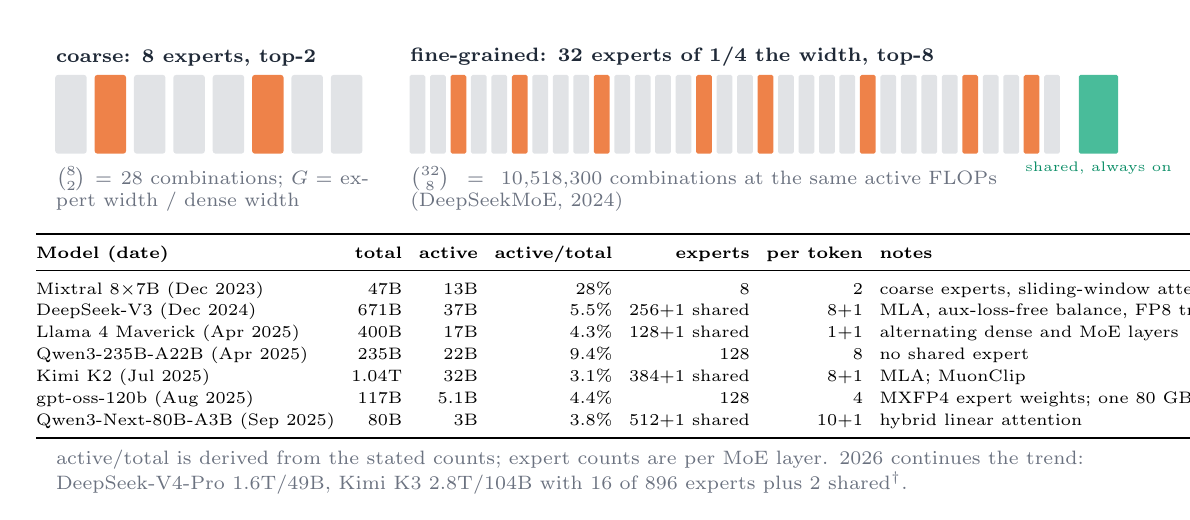
\begin{tikzpicture}
  \useasboundingbox (0,0) rectangle (14.4,5.9);
  % (a) coarse
  \node[lab,anchor=south west,font=\scriptsize\bfseries,text=ink] at (0.3,5.35) {coarse: 8 experts, top-2};
  \foreach \i in {0,...,7}{
    \pgfmathtruncatemacro{\act}{ifthenelse(\i==1||\i==5,1,0)}
    \ifnum\act=1 \fill[attn!75,rounded corners=1pt] ({0.35+\i*0.5},4.3) rectangle ++(0.4,1.0);
    \else \fill[muted!20,rounded corners=1pt] ({0.35+\i*0.5},4.3) rectangle ++(0.4,1.0); \fi}
  \node[lab,anchor=north west,text width=4.2cm] at (0.3,4.2) {$\binom{8}{2}=28$ combinations; $G$ = expert width / dense width};
  % (b) fine-grained
  \node[lab,anchor=south west,font=\scriptsize\bfseries,text=ink] at (4.8,5.35) {fine-grained: 32 experts of 1/4 the width, top-8};
  \foreach \i in {0,...,31}{
    \pgfmathtruncatemacro{\act}{ifthenelse(\i==2||\i==5||\i==9||\i==14||\i==17||\i==22||\i==27||\i==30,1,0)}
    \ifnum\act=1 \fill[attn!75,rounded corners=0.6pt] ({4.85+\i*0.26},4.3) rectangle ++(0.2,1.0);
    \else \fill[muted!20,rounded corners=0.6pt] ({4.85+\i*0.26},4.3) rectangle ++(0.2,1.0); \fi}
  \fill[emb!75,rounded corners=0.6pt] (13.35,4.3) rectangle ++(0.5,1.0);
  \node[lab,anchor=north,font=\tiny,text=emb!85!black] at (13.6,4.25) {shared, always on};
  \node[lab,anchor=north west,text width=8.4cm] at (4.8,4.2) {$\binom{32}{8}=10{,}518{,}300$ combinations at the same active FLOPs (DeepSeekMoE, 2024)};
  \node[anchor=north west,inner sep=0,font=\fontsize{6.1}{7.2}\selectfont] at (0.1,3.3) {%
    \renewcommand{\arraystretch}{1.1}\setlength{\tabcolsep}{3pt}%
    \begin{tabular}{@{}lrrrrrl@{}}
      \toprule
      \textbf{Model (date)} & \textbf{total} & \textbf{active} & \textbf{active/total} & \textbf{experts} & \textbf{per token} & \textbf{notes}\\
      \midrule
      Mixtral 8$\times$7B (Dec 2023) & 47B & 13B & 28\% & 8 & 2 & coarse experts, sliding-window attention\\
      DeepSeek-V3 (Dec 2024) & 671B & 37B & 5.5\% & 256+1 shared & 8+1 & MLA, aux-loss-free balance, FP8 training\\
      Llama 4 Maverick (Apr 2025) & 400B & 17B & 4.3\% & 128+1 shared & 1+1 & alternating dense and MoE layers\\
      Qwen3-235B-A22B (Apr 2025) & 235B & 22B & 9.4\% & 128 & 8 & no shared expert\\
      Kimi K2 (Jul 2025) & 1.04T & 32B & 3.1\% & 384+1 shared & 8+1 & MLA; MuonClip\\
      gpt-oss-120b (Aug 2025) & 117B & 5.1B & 4.4\% & 128 & 4 & MXFP4 expert weights; one 80 GB GPU\\
      Qwen3-Next-80B-A3B (Sep 2025) & 80B & 3B & 3.8\% & 512+1 shared & 10+1 & hybrid linear attention\\
      \bottomrule
    \end{tabular}};
  \node[lab,anchor=north west,text width=13.8cm] at (0.3,0.6) {active/total is derived from the stated counts; expert counts are per MoE layer. 2026 continues the trend: DeepSeek-V4-Pro 1.6T/49B, Kimi K3 2.8T/104B with 16 of 896 experts plus 2 shared$^\dagger$.};
\end{tikzpicture}
\end{frame}

% ---------------------------------------------------------------- 7
\begin{frame}{MoE systems: expert parallelism, all-to-all, and the memory bill}
\framesubtitle{The experts live on different GPUs; every MoE layer is two network shuffles around a small matmul.}
\centering
\begin{tikzpicture}
  \useasboundingbox (0,0) rectangle (14.4,5.9);
  \foreach \i in {0,...,3}{
    \node[comp=tok,minimum width=2.0cm,minimum height=0.75cm,font=\scriptsize,align=center] (g\i) at ({1.3+\i*2.3},5.1) {\textbf{GPU \i}\\tokens, attention};
    \node[comp=attn,minimum width=2.0cm,minimum height=0.75cm,font=\scriptsize,align=center] (x\i) at ({1.3+\i*2.3},3.3) {\textbf{experts} $E_{\the\numexpr\i*2\relax}$, $E_{\the\numexpr\i*2+1\relax}$};}
  \foreach \i in {0,...,3}{\foreach \j in {0,...,3}{
    \draw[thinflow,draw=ink!30] ([yshift=-1pt]g\i.south) -- ([yshift=1pt]x\j.north);}}
  \node[lab,anchor=east,align=right] at (0.25,4.2) {dispatch\\all-to-all};
  \node[lab,anchor=west,align=left] at (9.35,4.2) {then combine\\all-to-all back};
  \node[lab,anchor=north,text width=11.0cm,align=center] at (5.6,2.85) {each token travels to its $k$ experts' GPUs and back, twice per layer; DeepSeek-V3 caps each token at $M=4$ nodes and overlaps the shuffles with compute (DualPipe).};
  \foreach \x/\c/\ttl/\body in {
      0.2/attn/{Memory, not FLOPs}/{All experts stay resident: 671B weights at one byte each is 671 GB, on eight or more GPUs, to run 37B of compute per token. MoE buys FLOPs with memory.},
      4.95/attn/{Decode batching}/{At batch 1 a token reads only its $k$ experts, so bytes per token fall with the active fraction. A large batch touches every expert, and the layer looks dense again.},
      9.7/attn/{Load at inference}/{Expert popularity is uneven per domain; serving systems replicate hot experts, or place them so that each GPU's traffic is similar (DeepSeek's redundant experts).}}{
    \node[anchor=north west,inner sep=0] at (\x,2.05) {%
      \begin{tikzpicture}
        \node[anchor=north west,text width=4.25cm,align=flush left,font=\scriptsize,text=ink,minimum height=1.9cm,
              inner xsep=6pt,inner ysep=5pt,rounded corners=3pt,fill=\c!8] (c)
              {{\color{\c}\bfseries\ttl}\\[2pt]\body};
      \end{tikzpicture}};}
  \node[lab,anchor=west,text=posc!85!black,font=\scriptsize\bfseries] at (10.9,5.1) {compute: $N_{\text{active}}$};
  \node[lab,anchor=west,text=posc!85!black,font=\scriptsize\bfseries] at (10.9,3.3) {memory: $N_{\text{total}}$};
\end{tikzpicture}
\end{frame}

% ---------------------------------------------------------------- 8
\begin{frame}{MoE scaling laws: how sparse should a model be?}
\framesubtitle{At a fixed training budget there is a best active fraction, and it falls as the total parameter count grows.}
\centering
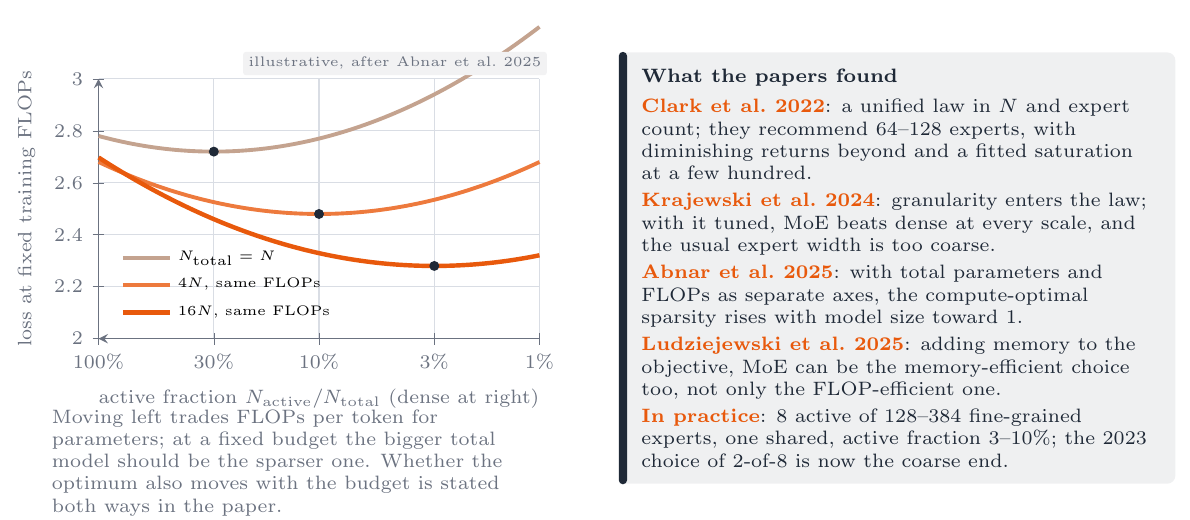
\begin{tikzpicture}
  \useasboundingbox (0,0) rectangle (14.4,5.9);
  \begin{axis}[lecture,at={(0.9cm,1.95cm)},anchor=south west,scale only axis,width=5.6cm,height=3.3cm,
      xmode=log,xmin=0.01,xmax=1,ymin=2.0,ymax=3.0,domain=0.01:1,samples=80,
      xtick={0.01,0.03,0.1,0.3,1},xticklabels={1\%,3\%,10\%,30\%,100\%},x dir=reverse,
      xlabel={active fraction $N_{\text{active}}/N_{\text{total}}$ (dense at right)},ylabel={loss at fixed training FLOPs},
      legend style={font=\tiny,at={(0.03,0.03)},anchor=south west}]
    \addplot[trn!60,line width=1.4pt] {2.72+0.22*(ln(x/0.3)/ln(10))^2}; \addlegendentry{$N_{\text{total}}=N$}
    \addplot[attn!80,line width=1.4pt] {2.48+0.2*(ln(x/0.1)/ln(10))^2}; \addlegendentry{$4N$, same FLOPs}
    \addplot[attn,line width=1.6pt] {2.28+0.18*(ln(x/0.03)/ln(10))^2}; \addlegendentry{$16N$, same FLOPs}
    \fill[ink] (axis cs:0.3,2.72) circle (1.8pt); \fill[ink] (axis cs:0.1,2.48) circle (1.8pt); \fill[ink] (axis cs:0.03,2.28) circle (1.8pt);
  \end{axis}
  \srctag{6.6}{5.6}{illustrative, after Abnar et al.\ 2025}
  \node[txt,anchor=north west,text width=6.3cm,font=\scriptsize,text=muted] at (0.3,1.05)
    {Moving left trades FLOPs per token for parameters; at a fixed budget the bigger total model should be the sparser one. Whether the optimum also moves with the budget is stated both ways in the paper.};
  \bgpanels{7.5}{5.6}{6.5cm}{What the papers found}{%
    \hl{attn}{Clark et al.\ 2022}: a unified law in $N$ and expert count;
    they recommend 64--128 experts, with diminishing returns beyond and a
    fitted saturation at a few hundred.\\[2pt]
    \hl{attn}{Krajewski et al.\ 2024}: granularity enters the law; with it tuned,
    MoE beats dense at every scale, and the usual expert width is too coarse.\\[2pt]
    \hl{attn}{Abnar et al.\ 2025}: with total parameters and FLOPs as separate
    axes, the compute-optimal sparsity rises with model size toward 1.\\[2pt]
    \hl{attn}{Ludziejewski et al.\ 2025}: adding memory to the objective, MoE
    can be the memory-efficient choice too, not only the FLOP-efficient one.\\[2pt]
    \hl{attn}{In practice}: 8 active of 128--384 fine-grained experts, one shared,
    active fraction 3--10\%; the 2023 choice of 2-of-8 is now the coarse end.}
\end{tikzpicture}
\end{frame}

% ---------------------------------------------------------------- 9
\begin{frame}{A worked bill: DeepSeek-V3 against a dense model}
\framesubtitle{Sparsity in the experts, compression in the attention, FP8 everywhere: the three levers in one model.}
\centering
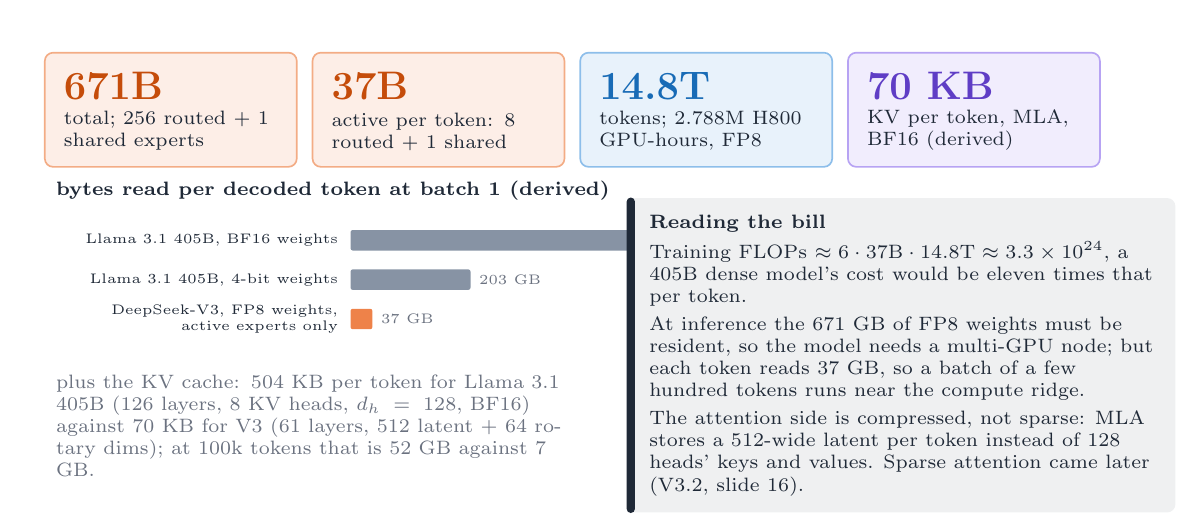
\begin{tikzpicture}
  \useasboundingbox (0,0) rectangle (14.4,5.9);
  \stat{0.2}{5.6}{671B}{total; 256 routed + 1 shared experts}{attn}
  \stat{3.6}{5.6}{37B}{active per token: 8 routed + 1 shared}{attn}
  \stat{7.0}{5.6}{14.8T}{tokens; 2.788M H800 GPU-hours, FP8}{mlp}
  \stat{10.4}{5.6}{70 KB}{KV per token, MLA, BF16 (derived)}{posc}
  % bytes per token bar chart
  \node[lab,anchor=south west,font=\scriptsize\bfseries,text=ink] at (0.3,3.65) {bytes read per decoded token at batch 1 (derived)};
  \foreach \i/\n/\v/\c in {0/{Llama 3.1 405B, BF16 weights}/810/tok,1/{Llama 3.1 405B, 4-bit weights}/203/tok,2/{DeepSeek-V3, FP8 weights, active experts only}/37/attn}{
    \node[lab,anchor=east,font=\tiny,text=ink,text width=3.6cm,align=right] at (4.0,{3.2-\i*0.5}) {\n};
    \barh{4.1}{3.2-\i*0.5}{\v*0.0075}{\c!75}
    \node[lab,anchor=west,font=\tiny] at ({4.15+\v*0.0075},{3.2-\i*0.5}) {\v\ GB};}
  \node[lab,anchor=north west,text width=6.6cm] at (0.3,1.55) {plus the KV cache: 504 KB per token for Llama 3.1 405B (126 layers, 8 KV heads, $d_h=128$, BF16) against 70 KB for V3 (61 layers, 512 latent + 64 rotary dims); at 100k tokens that is 52 GB against 7 GB.};
  \bgpanels{7.6}{3.75}{6.4cm}{Reading the bill}{%
    Training FLOPs $\approx6\cdot37\text{B}\cdot14.8\text{T}\approx3.3\times10^{24}$, a
    405B dense model's cost would be eleven times that per token.\\[2pt]
    At inference the 671 GB of FP8 weights must be resident, so the model
    needs a multi-GPU node; but each token reads 37 GB, so a batch of a few
    hundred tokens runs near the compute ridge.\\[2pt]
    The attention side is compressed, not sparse: MLA stores a 512-wide
    latent per token instead of 128 heads' keys and values. Sparse
    attention came later (V3.2, slide 16).}
\end{tikzpicture}
\end{frame}

% ---------------------------------------------------------------- 10
\stage{3}
\begin{frame}{Weight pruning: the classics}
\framesubtitle{Remove the weights that matter least, retrain, repeat. Most of a trained network is slack; the last 10\% is not.}
\centering
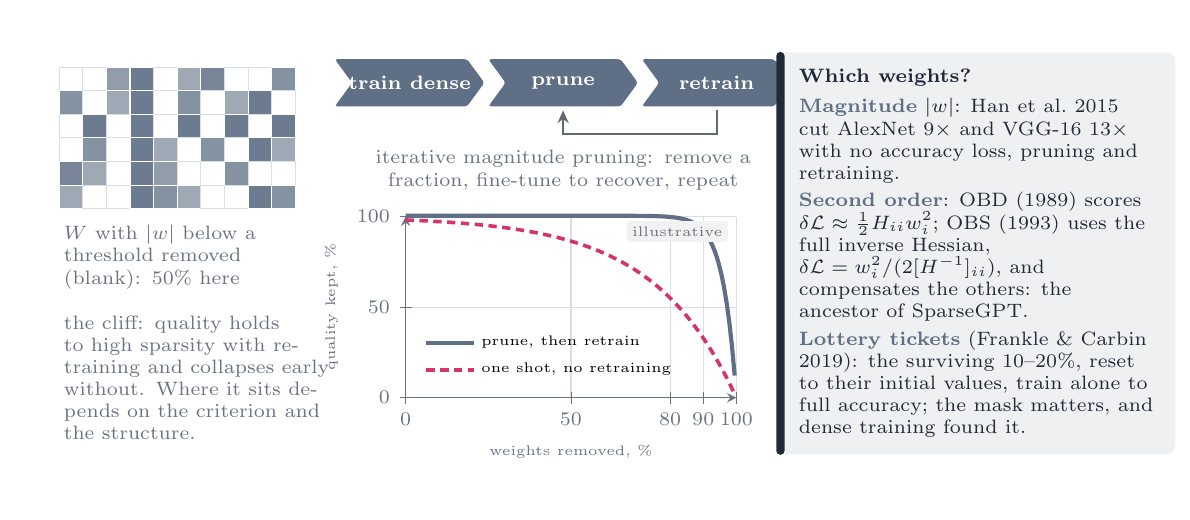
\begin{tikzpicture}
  \useasboundingbox (0,0) rectangle (14.4,5.9);
  % weight grid with magnitude shading; small ones pruned
  \foreach \r in {0,...,5}{\foreach \c in {0,...,9}{
    \pgfmathtruncatemacro{\mag}{mod(\r*37+\c*53+\r*\c*11,10)}
    \pgfmathtruncatemacro{\sh}{20+\mag*8}
    \ifnum\mag>4
      \fill[tok!\sh!white,draw=paper,line width=0.4pt] ({0.4+\c*0.3},{5.1-\r*0.3}) rectangle ++(0.3,0.3);
    \else
      \draw[hair,line width=0.3pt] ({0.4+\c*0.3},{5.1-\r*0.3}) rectangle ++(0.3,0.3);
    \fi}}
  \node[lab,anchor=north west,text width=3.3cm] at (0.4,3.45) {$W$ with $|w|$ below a threshold removed (blank): 50\% here};
  \chev{3.9}{4.9}{1.9}{tok}{train dense}
  \chev{5.85}{4.9}{1.9}{tok}{prune}
  \chev{7.8}{4.9}{1.9}{tok}{retrain}
  \draw[flow] (8.75,4.85) -- (8.75,4.55) -| (6.8,4.85);
  \node[lab,anchor=north,text width=5.8cm,align=center] at (6.8,4.4) {iterative magnitude pruning: remove a fraction, fine-tune to recover, repeat};
  % accuracy vs sparsity
  \begin{axis}[lecture,at={(4.8cm,1.2cm)},anchor=south west,scale only axis,width=4.2cm,height=2.3cm,
      xmin=0,xmax=100,ymin=0,ymax=100,domain=0:99.5,samples=120,xtick={0,50,80,90,100},ytick={0,50,100},
      xlabel={weights removed, \%},ylabel={quality kept, \%},x label style={font=\tiny},y label style={font=\tiny},
      legend style={font=\tiny,at={(0.03,0.05)},anchor=south west}]
    \addplot[tok,line width=1.5pt] {100-100*exp(-(100-x)/4)+0.5}; \addlegendentry{prune, then retrain}
    \addplot[outc,densely dashed,line width=1.3pt] {100-100*exp(-(100-x)/25)}; \addlegendentry{one shot, no retraining}
  \end{axis}
  \srctag{8.9}{3.45}{illustrative}
  \node[lab,anchor=north west,text width=3.4cm] at (0.4,2.3) {the cliff: quality holds to high sparsity with retraining and collapses early without. Where it sits depends on the criterion and the structure.};
  \bgpanels{9.5}{5.6}{4.5cm}{Which weights?}{%
    \hl{tok}{Magnitude} $|w|$: Han et al.\ 2015 cut AlexNet 9$\times$ and VGG-16
    13$\times$ with no accuracy loss, pruning and retraining.\\[2pt]
    \hl{tok}{Second order}: OBD (1989) scores
    $\delta\mathcal{L}\approx\tfrac12 H_{ii}w_i^2$; OBS (1993) uses the full
    inverse Hessian, $\delta\mathcal{L}=w_i^2/(2[H^{-1}]_{ii})$, and
    compensates the others: the ancestor of SparseGPT.\\[2pt]
    \hl{tok}{Lottery tickets} (Frankle \& Carbin 2019): the surviving 10--20\%,
    reset to their initial values, train alone to full accuracy; the
    mask matters, and dense training found it.}
\end{tikzpicture}
\end{frame}

% ---------------------------------------------------------------- 11
\begin{frame}{Structure decides the speedup}
\framesubtitle{A zero only saves time if the hardware can skip it. Unstructured zeros rarely do on a GPU; 2:4 and whole blocks do.}
\centering
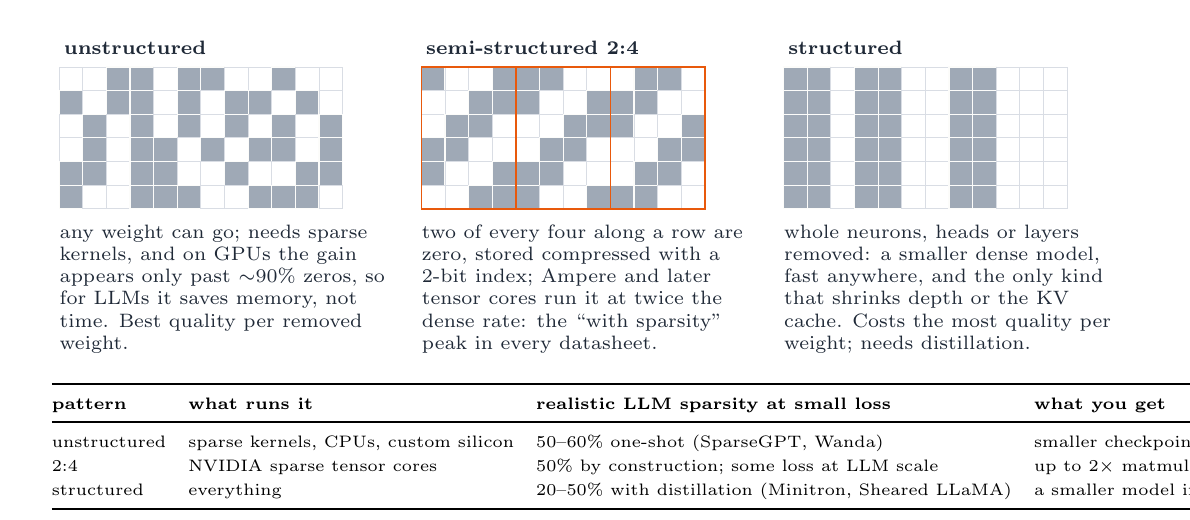
\begin{tikzpicture}
  \useasboundingbox (0,0) rectangle (14.4,5.9);
  \foreach \k/\x/\ttl in {0/0.4/{unstructured},1/5.0/{semi-structured 2:4},2/9.6/{structured}}{
    \node[lab,anchor=south west,font=\scriptsize\bfseries,text=ink] at (\x,5.5) {\ttl};
    \foreach \r in {0,...,5}{\foreach \c in {0,...,11}{
      \ifnum\k=0 \pgfmathtruncatemacro{\on}{mod(\r*37+\c*53+\r*\c*11,10)>4}\fi
      \ifnum\k=1 \pgfmathtruncatemacro{\on}{ifthenelse(mod(\r*7+\c*3+int(\c/4)*5,4)<2,1,0)}\fi
      \ifnum\k=2 \pgfmathtruncatemacro{\on}{ifthenelse(\c==2||\c==5||\c==6||\c==9||\c==10||\c==11,0,1)}\fi
      \ifnum\on=1
        \fill[tok!60!white,draw=paper,line width=0.4pt] ({\x+\c*0.3},{5.1-\r*0.3}) rectangle ++(0.3,0.3);
      \else
        \draw[hair,line width=0.3pt] ({\x+\c*0.3},{5.1-\r*0.3}) rectangle ++(0.3,0.3);
      \fi}}}
  \foreach \c in {0,4,8}{\draw[attn,line width=0.6pt] ({5.0+\c*0.3},5.4) rectangle ++(1.2,-1.8);}
  \foreach \x/\body in {0.4/{any weight can go; needs sparse kernels, and on GPUs the gain appears only past $\sim$90\% zeros, so for LLMs it saves memory, not time. Best quality per removed weight.},
                        5.0/{two of every four along a row are zero, stored compressed with a 2-bit index; Ampere and later tensor cores run it at twice the dense rate: the ``with sparsity'' peak in every datasheet.},
                        9.6/{whole neurons, heads or layers removed: a smaller dense model, fast anywhere, and the only kind that shrinks depth or the KV cache. Costs the most quality per weight; needs distillation.}}{
    \node[txt,anchor=north west,text width=4.3cm,font=\scriptsize] at (\x,3.4) {\body};}
  \node[anchor=north west,inner sep=0,font=\fontsize{6.3}{7.6}\selectfont] at (0.3,1.4) {%
    \renewcommand{\arraystretch}{1.15}\setlength{\tabcolsep}{4pt}%
    \begin{tabular}{@{}llll@{}}
      \toprule
      \textbf{pattern} & \textbf{what runs it} & \textbf{realistic LLM sparsity at small loss} & \textbf{what you get}\\
      \midrule
      unstructured & sparse kernels, CPUs, custom silicon & 50--60\% one-shot (SparseGPT, Wanda) & smaller checkpoint; little GPU speedup\\
      2:4 & NVIDIA sparse tensor cores & 50\% by construction; some loss at LLM scale & up to 2$\times$ matmul, $\sim$1.3--1.5$\times$ end to end\\
      structured & everything & 20--50\% with distillation (Minitron, Sheared LLaMA) & a smaller model in every dimension\\
      \bottomrule
    \end{tabular}};
\end{tikzpicture}
\end{frame}

% ---------------------------------------------------------------- 12
\begin{frame}{One-shot pruning at LLM scale: SparseGPT and Wanda}
\framesubtitle{No retraining: prune one layer at a time so that its outputs on a few calibration samples barely change.}
\centering
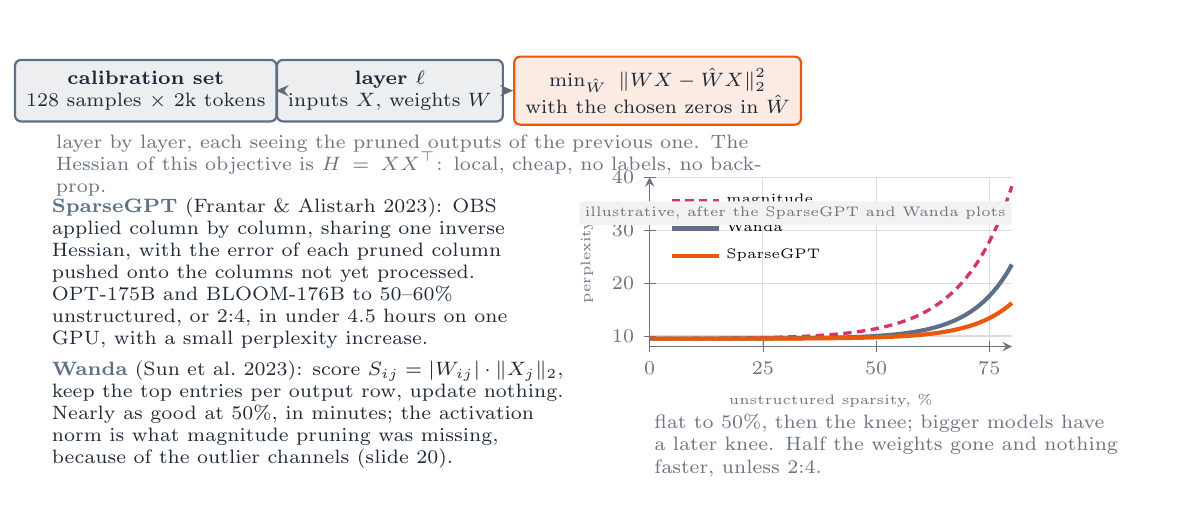
\begin{tikzpicture}
  \useasboundingbox (0,0) rectangle (14.4,5.9);
  \node[comp=tok,minimum width=2.3cm,minimum height=0.7cm,font=\scriptsize,align=center] (cal) at (1.5,5.1) {\textbf{calibration set}\\128 samples $\times$ 2k tokens};
  \node[comp=tok,minimum width=2.3cm,minimum height=0.7cm,font=\scriptsize,align=center] (lay) at (4.6,5.1) {\textbf{layer $\ell$}\\inputs $X$, weights $W$};
  \node[comp=attn,minimum width=2.6cm,minimum height=0.7cm,font=\scriptsize,align=center] (obj) at (8.0,5.1) {$\min_{\hat W}\ \|WX-\hat W X\|_2^2$\\with the chosen zeros in $\hat W$};
  \draw[flow] (cal) -- (lay); \draw[flow] (lay) -- (obj);
  \node[lab,anchor=north west,text width=9.4cm] at (0.3,4.6) {layer by layer, each seeing the pruned outputs of the previous one. The Hessian of this objective is $H=XX^\top$: local, cheap, no labels, no backprop.};
  \node[txt,anchor=north west,text width=6.5cm,font=\scriptsize] at (0.3,3.75) {%
    \hl{tok}{SparseGPT} (Frantar \& Alistarh 2023): OBS applied column by column,
    sharing one inverse Hessian, with the error of each pruned column
    pushed onto the columns not yet processed. OPT-175B and BLOOM-176B to
    50--60\% unstructured, or 2:4, in under 4.5 hours on one GPU, with a
    small perplexity increase.\\[3pt]
    \hl{tok}{Wanda} (Sun et al.\ 2023): score $S_{ij}=|W_{ij}|\cdot\|X_j\|_2$,
    keep the top entries per output row, update nothing. Nearly as good at
    50\%, in minutes; the activation norm is what magnitude pruning was
    missing, because of the outlier channels (slide 20).};
  \begin{axis}[lecture,at={(7.9cm,1.85cm)},anchor=south west,scale only axis,width=4.6cm,height=2.15cm,
      xmin=0,xmax=80,ymin=8,ymax=40,domain=0:80,samples=80,xtick={0,25,50,75},ytick={10,20,30,40},
      xlabel={unstructured sparsity, \%},ylabel={perplexity},x label style={font=\tiny},y label style={font=\tiny},
      legend style={font=\tiny,at={(0.03,0.97)},anchor=north west}]
    \addplot[outc,densely dashed,line width=1.2pt] {9.5+0.02*exp(x/11)}; \addlegendentry{magnitude}
    \addplot[tok,line width=1.5pt] {9.5+0.5*exp((x-50)/9)}; \addlegendentry{Wanda}
    \addplot[attn,line width=1.5pt] {9.5+0.3*exp((x-52)/9)}; \addlegendentry{SparseGPT}
  \end{axis}
  \srctag{12.5}{3.7}{illustrative, after the SparseGPT and Wanda plots}
  \node[lab,anchor=north west,text width=6.3cm] at (7.9,1.05) {flat to 50\%, then the knee; bigger models have a later knee. Half the weights gone and nothing faster, unless 2:4.};
\end{tikzpicture}
\end{frame}

% ---------------------------------------------------------------- 13
\begin{frame}{Pruning with distillation, and a law for sparsity}
\framesubtitle{The cheap way to a small model is to cut a big one down and teach it from its parent, not to train from scratch.}
\centering
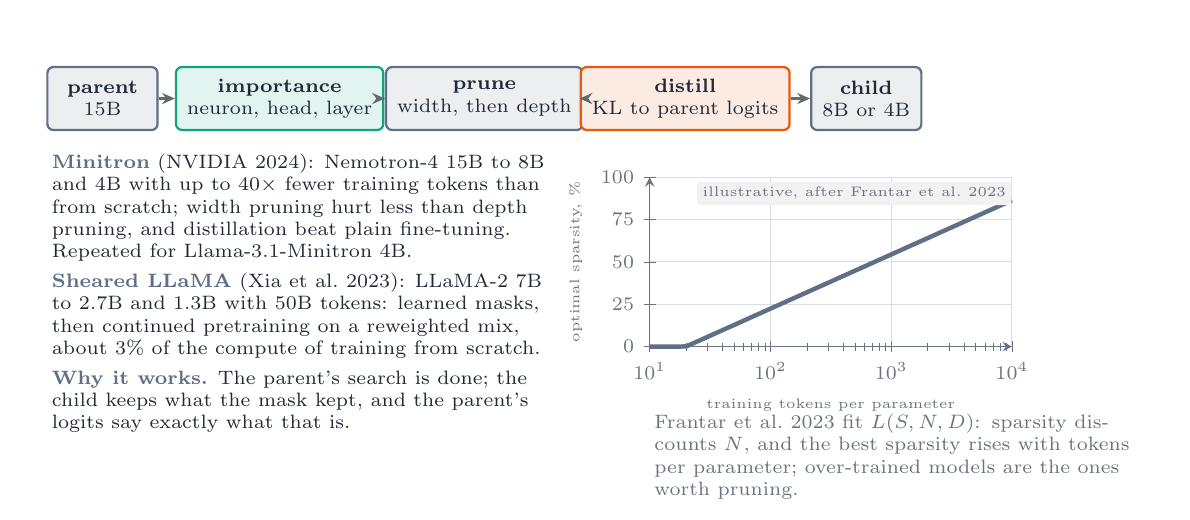
\begin{tikzpicture}
  \useasboundingbox (0,0) rectangle (14.4,5.9);
  \node[comp=tok,minimum width=1.4cm,minimum height=0.8cm,font=\scriptsize,align=center] (par) at (0.95,5.0) {\textbf{parent}\\15B};
  \node[comp=emb,minimum width=2.2cm,minimum height=0.8cm,font=\scriptsize,align=center] (imp) at (3.2,5.0) {\textbf{importance}\\neuron, head, layer};
  \node[comp=tok,minimum width=1.9cm,minimum height=0.8cm,font=\scriptsize,align=center] (pr) at (5.8,5.0) {\textbf{prune}\\width, then depth};
  \node[comp=attn,minimum width=2.2cm,minimum height=0.8cm,font=\scriptsize,align=center] (ds) at (8.35,5.0) {\textbf{distill}\\KL to parent logits};
  \node[comp=tok,minimum width=1.4cm,minimum height=0.8cm,font=\scriptsize,align=center] (ch) at (10.65,5.0) {\textbf{child}\\8B or 4B};
  \draw[flow] (par) -- (imp); \draw[flow] (imp) -- (pr); \draw[flow] (pr) -- (ds); \draw[flow] (ds) -- (ch);
  \node[txt,anchor=north west,text width=6.5cm,font=\scriptsize] at (0.3,4.3) {%
    \hl{tok}{Minitron} (NVIDIA 2024): Nemotron-4 15B to 8B and 4B with up to
    40$\times$ fewer training tokens than from scratch; width pruning hurt
    less than depth pruning, and distillation beat plain fine-tuning.
    Repeated for Llama-3.1-Minitron 4B.\\[3pt]
    \hl{tok}{Sheared LLaMA} (Xia et al.\ 2023): LLaMA-2 7B to 2.7B and 1.3B
    with 50B tokens: learned masks, then continued pretraining on a
    reweighted mix, about 3\% of the compute of training from scratch.\\[3pt]
    \hl{tok}{Why it works.} The parent's search is done; the child keeps
    what the mask kept, and the parent's logits say exactly what that is.};
  \begin{axis}[lecture,at={(7.9cm,1.85cm)},anchor=south west,scale only axis,width=4.6cm,height=2.15cm,
      xmode=log,xmin=10,xmax=10000,ymin=0,ymax=100,domain=10:10000,samples=60,xtick={10,100,1000,10000},ytick={0,25,50,75,100},
      xlabel={training tokens per parameter},ylabel={optimal sparsity, \%},x label style={font=\tiny},y label style={font=\tiny}]
    \addplot[tok,line width=1.6pt] {min(90,max(0,32*(ln(x)/ln(10)-1.3)))};
  \end{axis}
  \srctag{12.5}{3.95}{illustrative, after Frantar et al.\ 2023}
  \node[lab,anchor=north west,text width=6.4cm] at (7.9,1.05) {Frantar et al.\ 2023 fit $L(S,N,D)$: sparsity discounts $N$, and the best sparsity rises with tokens per parameter; over-trained models are the ones worth pruning.};
\end{tikzpicture}
\end{frame}

% ---------------------------------------------------------------- 14
\stage{4}
\begin{frame}{Activation sparsity: most neurons are silent for most tokens}
\framesubtitle{In a ReLU MLP over 90\% of the hidden units are zero per input; skip their rows and the layer is almost free.}
\centering
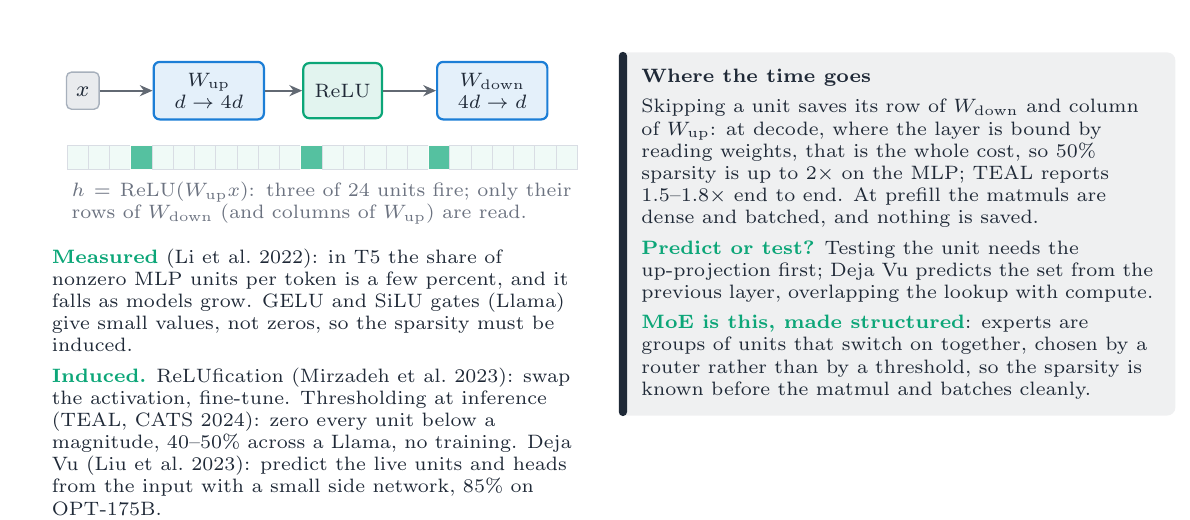
\begin{tikzpicture}
  \useasboundingbox (0,0) rectangle (14.4,5.9);
  \node[chip,fill=tok!14,draw=tok!55] (x) at (0.7,5.1) {$x$};
  \node[comp=mlp,minimum width=1.4cm,minimum height=0.7cm,font=\scriptsize,align=center] (up) at (2.3,5.1) {$W_{\text{up}}$\\$d\to4d$};
  \node[comp=emb,minimum width=1.0cm,minimum height=0.7cm,font=\scriptsize] (act) at (4.0,5.1) {ReLU};
  \node[comp=mlp,minimum width=1.4cm,minimum height=0.7cm,font=\scriptsize,align=center] (dn) at (5.9,5.1) {$W_{\text{down}}$\\$4d\to d$};
  \draw[flow] (x) -- (up); \draw[flow] (up) -- (act); \draw[flow] (act) -- (dn);
  % hidden vector strip
  \foreach \i in {0,...,23}{
    \pgfmathtruncatemacro{\on}{ifthenelse(\i==3||\i==11||\i==17,1,0)}
    \ifnum\on=1 \fill[emb!70,draw=paper,line width=0.4pt] ({0.5+\i*0.27},4.1) rectangle ++(0.27,0.3);
    \else \fill[emb!6,draw=hair,line width=0.3pt] ({0.5+\i*0.27},4.1) rectangle ++(0.27,0.3); \fi}
  \node[lab,anchor=north west,text width=6.6cm] at (0.5,4.0) {$h=\mathrm{ReLU}(W_{\text{up}}x)$: three of 24 units fire; only their rows of $W_{\text{down}}$ (and columns of $W_{\text{up}}$) are read.};
  \node[txt,anchor=north west,text width=6.6cm,font=\scriptsize] at (0.3,3.1) {%
    \hl{emb}{Measured} (Li et al.\ 2022): in T5 the share of nonzero MLP units
    per token is a few percent, and it falls as models grow. GELU and SiLU
    gates (Llama) give small values, not zeros, so the sparsity must be induced.\\[3pt]
    \hl{emb}{Induced.} ReLUfication (Mirzadeh et al.\ 2023): swap the activation,
    fine-tune. Thresholding at inference (TEAL, CATS 2024): zero every unit
    below a magnitude, 40--50\% across a Llama, no training. Deja Vu (Liu et al.\
    2023): predict the live units and heads from the input with a small side
    network, 85\% on OPT-175B.};
  \bgpanels{7.5}{5.6}{6.5cm}{Where the time goes}{%
    Skipping a unit saves its row of $W_{\text{down}}$ and column of
    $W_{\text{up}}$: at decode, where the layer is bound by reading weights,
    that is the whole cost, so 50\% sparsity is up to 2$\times$ on the MLP;
    TEAL reports 1.5--1.8$\times$ end to end. At prefill the matmuls are
    dense and batched, and nothing is saved.\\[3pt]
    \hl{emb}{Predict or test?} Testing the unit needs the up-projection
    first; Deja Vu predicts the set from the previous layer, overlapping
    the lookup with compute.\\[3pt]
    \hl{emb}{MoE is this, made structured}: experts are groups of units that
    switch on together, chosen by a router rather than by a threshold, so
    the sparsity is known before the matmul and batches cleanly.}
\end{tikzpicture}
\end{frame}

% ---------------------------------------------------------------- 15
\begin{frame}{Attention: where the cost is, and the KV cache}
\framesubtitle{Prefill is quadratic in length; decode reads the whole cache per token. Both are attacked by sharing and by sparsity.}
\centering
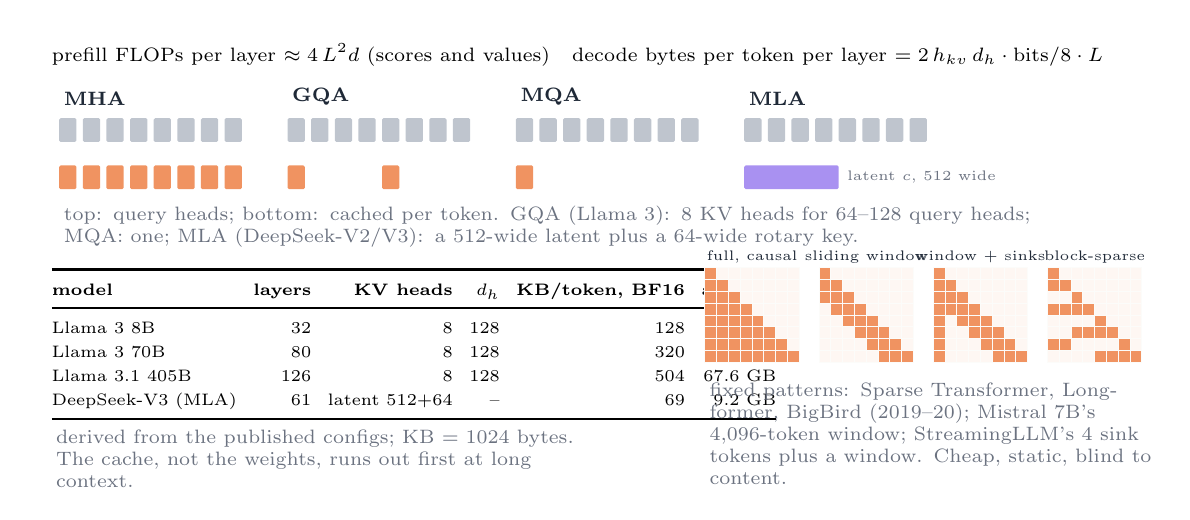
\begin{tikzpicture}
  \useasboundingbox (0,0) rectangle (14.4,5.9);
  \node[anchor=north west,inner sep=0,font=\scriptsize,align=left] at (0.3,5.7)
    {prefill FLOPs per layer $\approx 4\,L^2 d$ (scores and values)\quad decode bytes per token per layer $=2\,h_{kv}\,d_h\cdot\text{bits}/8\cdot L$};
  % head-sharing diagram
  \foreach \k/\x/\ttl/\hk/\c in {0/0.4/{MHA}/8/attn,1/3.3/{GQA}/2/attn,2/6.2/{MQA}/1/attn,3/9.1/{MLA}/0/posc}{
    \node[lab,anchor=south west,font=\scriptsize\bfseries,text=ink] at (\x,4.85) {\ttl};
    \foreach \i in {0,...,7}{\fill[tok!40,rounded corners=0.5pt] ({\x+\i*0.3},4.45) rectangle ++(0.22,0.3);}
    \ifnum\k=3
      \fill[posc!60,rounded corners=0.5pt] (\x,3.85) rectangle ++(1.2,0.3);
      \node[lab,anchor=west,font=\tiny] at (\x+1.25,4.0) {latent $c$, 512 wide};
    \else
      \pgfmathsetmacro{\stp}{2.4/\hk}
      \foreach \j in {1,...,\hk}{\fill[\c!65,rounded corners=0.5pt] ({\x+(\j-1)*\stp},3.85) rectangle ++(0.22,0.3);}
    \fi}
  \node[lab,anchor=north west,text width=12.5cm] at (0.4,3.7) {top: query heads; bottom: cached per token. GQA (Llama 3): 8 KV heads for 64--128 query heads; MQA: one; MLA (DeepSeek-V2/V3): a 512-wide latent plus a 64-wide rotary key.};
  \node[anchor=north west,inner sep=0,font=\fontsize{6.3}{7.6}\selectfont] at (0.3,2.85) {%
    \renewcommand{\arraystretch}{1.15}\setlength{\tabcolsep}{3pt}%
    \begin{tabular}{@{}lrrrrr@{}}
      \toprule
      \textbf{model} & \textbf{layers} & \textbf{KV heads} & \textbf{$d_h$} & \textbf{KB/token, BF16} & \textbf{at 128k}\\
      \midrule
      Llama 3 8B & 32 & 8 & 128 & 128 & 17.2 GB\\
      Llama 3 70B & 80 & 8 & 128 & 320 & 42.9 GB\\
      Llama 3.1 405B & 126 & 8 & 128 & 504 & 67.6 GB\\
      DeepSeek-V3 (MLA) & 61 & latent 512+64 & -- & 69 & 9.2 GB\\
      \bottomrule
    \end{tabular}};
  \node[lab,anchor=north west,text width=6.6cm] at (0.3,0.85) {derived from the published configs; KB $=1024$ bytes. The cache, not the weights, runs out first at long context.};
  % mask patterns
  \foreach \k/\x/\ttl in {0/8.6/{full, causal},1/10.05/{sliding window},2/11.5/{window + sinks},3/12.95/{block-sparse}}{
    \node[lab,anchor=south,font=\tiny,text=ink] at (\x+0.6,2.85) {\ttl};
    \foreach \r in {0,...,7}{\foreach \c in {0,...,7}{
      \ifnum\k=0 \pgfmathtruncatemacro{\on}{\c<=\r}\fi
      \ifnum\k=1 \pgfmathtruncatemacro{\on}{\c<=\r&&\c>\r-3}\fi
      \ifnum\k=2 \pgfmathtruncatemacro{\on}{(\c<=\r&&\c>\r-3)||\c==0}\fi
      \ifnum\k=3 \pgfmathtruncatemacro{\on}{\c<=\r&&(int(\c/2)==int(\r/2)||mod(int(\c/2)+\r,3)==0)}\fi
      \ifnum\on=1 \fill[attn!65,draw=paper,line width=0.3pt] ({\x+\c*0.15},{2.7-\r*0.15}) rectangle ++(0.15,0.15);
      \else \fill[attn!5,draw=paper,line width=0.3pt] ({\x+\c*0.15},{2.7-\r*0.15}) rectangle ++(0.15,0.15); \fi}}}
  \node[lab,anchor=north west,text width=5.7cm] at (8.6,1.45) {fixed patterns: Sparse Transformer, Longformer, BigBird (2019--20); Mistral 7B's 4,096-token window; StreamingLLM's 4 sink tokens plus a window. Cheap, static, blind to content.};
\end{tikzpicture}
\end{frame}

% ---------------------------------------------------------------- 16
\begin{frame}{Learned sparse attention: pick the tokens that matter}
\framesubtitle{Score cheaply, attend fully to the top $k$: the 2025 designs make long context linear in what is read.}
\centering
\begin{tikzpicture}
  \useasboundingbox (0,0) rectangle (14.4,5.9);
  % DSA diagram
  \node[lab,anchor=south west,font=\scriptsize\bfseries,text=posc!85!black] at (0.3,5.5) {DeepSeek Sparse Attention (V3.2, 2025)};
  \node[chip,fill=attn!14,draw=attn!55] (q) at (0.7,4.75) {$q_t$};
  \node[comp=posc,minimum width=1.9cm,minimum height=0.65cm,font=\scriptsize,align=center] (idx) at (2.6,4.75) {\textbf{lightning indexer}\\few heads, FP8, all $t'<t$};
  \draw[flow] (q) -- (idx);
  \foreach \i in {0,...,19}{
    \pgfmathtruncatemacro{\on}{ifthenelse(\i==1||\i==4||\i==9||\i==13||\i==17||\i==18,1,0)}
    \pgfmathsetmacro{\bh}{0.1+0.5*mod(\i*7+3,5)/5}
    \ifnum\on=1 \fill[posc!75] ({4.1+\i*0.17},4.45) rectangle ++(0.12,{\bh+0.25});
    \else \fill[muted!35] ({4.1+\i*0.17},4.45) rectangle ++(0.12,\bh); \fi}
  \node[lab,anchor=north,text width=3.6cm,align=center,font=\tiny] at (5.8,4.4) {index scores over the cache; keep the top $k=2048$};
  \node[comp=attn,minimum width=1.7cm,minimum height=0.65cm,font=\scriptsize,align=center] (att) at (8.6,4.75) {\textbf{attention}\\over $k$ tokens only};
  \draw[flow] (7.55,4.75) -- (att);
  \node[lab,anchor=north west,text width=4.3cm] at (9.75,5.45) {per query: an $O(L)$ indexer with tiny heads, then $O(k)$ attention; memory unchanged, reads cut by $L/k$.};
  \node[lab,anchor=north west,text width=13.8cm] at (0.3,3.75) {Fixed patterns are blind to content. Eviction is cheap but irreversible: a dropped token is gone for every later query. Selection keeps everything and chooses per query, at the price of an indexer and a cache that still grows with $L$. Below $\sim$8k tokens dense attention is already cheap next to the MLPs; the gain is at decode and in long prefill.};
  \foreach \x/\c/\ttl/\body in {
      0.2/emb/{NSA (DeepSeek, Feb 2025)}/{Three branches summed with learned gates: compressed block summaries, the top-$n$ selected blocks, and a sliding window. Kernels written for the pattern; trained from scratch; large speedups at 64k on decode, forward and backward.},
      4.95/emb/{MoBA (Moonshot, Feb 2025)}/{The KV cache in blocks; each query is routed to its top blocks by a mean-key score, as a router routes tokens to experts. Switchable between full and sparse attention at inference.},
      9.7/emb/{Eviction, no training (2023--24)}/{H2O keeps the heavy-hitter tokens (20\% budget); StreamingLLM keeps the sinks and a window; SnapKV compresses the prompt's cache; Quest picks pages per query. Memory and reads both shrink.}}{
    \node[anchor=north west,inner sep=0] at (\x,2.6) {%
      \begin{tikzpicture}
        \node[anchor=north west,text width=4.25cm,align=flush left,font=\scriptsize,text=ink,minimum height=2.45cm,
              inner xsep=6pt,inner ysep=5pt,rounded corners=3pt,fill=\c!8] (c)
              {{\color{\c}\bfseries\ttl}\\[2pt]\body};
      \end{tikzpicture}};}
\end{tikzpicture}
\end{frame}

% ---------------------------------------------------------------- 17
\begin{frame}{The KV cache is where sparsity and precision meet}
\framesubtitle{Fewer heads, fewer bits, fewer tokens: the three multiply, and the cache at 128k goes from 43 GB to about 2.}
\centering
\begin{tikzpicture}
  \useasboundingbox (0,0) rectangle (14.4,5.9);
  \node[lab,anchor=south west,font=\scriptsize\bfseries,text=ink] at (0.3,5.55) {KV cache for one 128k-token sequence, Llama 3 70B (GQA, 8 KV heads), derived};
  \foreach \i/\n/\v/\c in {0/{BF16, every token}/42.9/tok,1/{FP8 (serving default)}/21.5/posc,2/{4-bit (KIVI-style)}/10.7/posc,3/{4-bit, 20\% of tokens kept (H2O-style)}/2.1/emb,4/{DeepSeek-V3, MLA, BF16, every token}/9.2/attn,5/{DeepSeek-V3, MLA, FP8}/4.6/attn}{
    \node[lab,anchor=east,font=\tiny,text=ink,text width=4.3cm,align=right] at (4.7,{5.2-\i*0.37}) {\n};
    \barh{4.8}{5.2-\i*0.37}{\v*0.17}{\c!75}
    \node[lab,anchor=west,font=\tiny] at ({4.85+\v*0.17},{5.2-\i*0.37}) {\v\ GB};}
  \node[lab,anchor=north west,text width=13.8cm] at (0.3,3.15) {eviction (H2O, SnapKV) shrinks memory and reads; selection (DSA, NSA, Quest) shrinks reads only, the cache still holds every token: at $k=2048$, V3.2 reads about 140 MB of latent per step instead of 9.2 GB (derived).};
  \foreach \x/\c/\ttl/\body in {
      0.2/posc/{Precision in the cache}/{FP8 keys and values are routine in vLLM and TensorRT-LLM. Keys carry outlier channels, so KIVI quantizes keys per channel and values per token, down to 2--4 bits.},
      4.95/emb/{Sparsity in the cache}/{Heads: GQA 8$\times$, MLA $\sim$7$\times$ over MHA. Tokens: eviction by attention mass (H2O, SnapKV) or per-query selection (Quest, DSA). 4-bit at a fifth of the tokens is 20$\times$.},
      9.7/attn/{What to expect}/{GQA plus FP8 covers most serving. Past 128k the cache dominates even at FP8; 2025--26 models add selection or MLA compression. Judge quality on long-context evals, not perplexity.}}{
    \node[anchor=north west,inner sep=0] at (\x,2.4) {%
      \begin{tikzpicture}
        \node[anchor=north west,text width=4.25cm,align=flush left,font=\scriptsize,text=ink,minimum height=2.2cm,
              inner xsep=6pt,inner ysep=4pt,rounded corners=3pt,fill=\c!8] (c)
              {{\color{\c}\bfseries\ttl}\\[2pt]\body};
      \end{tikzpicture}};}
\end{tikzpicture}
\end{frame}

% ---------------------------------------------------------------- 18
\stage{5}
\begin{frame}{Anatomy of a number}
\framesubtitle{Exponent bits buy range, mantissa bits buy precision; every format is a different split of a fixed budget.}
\centering
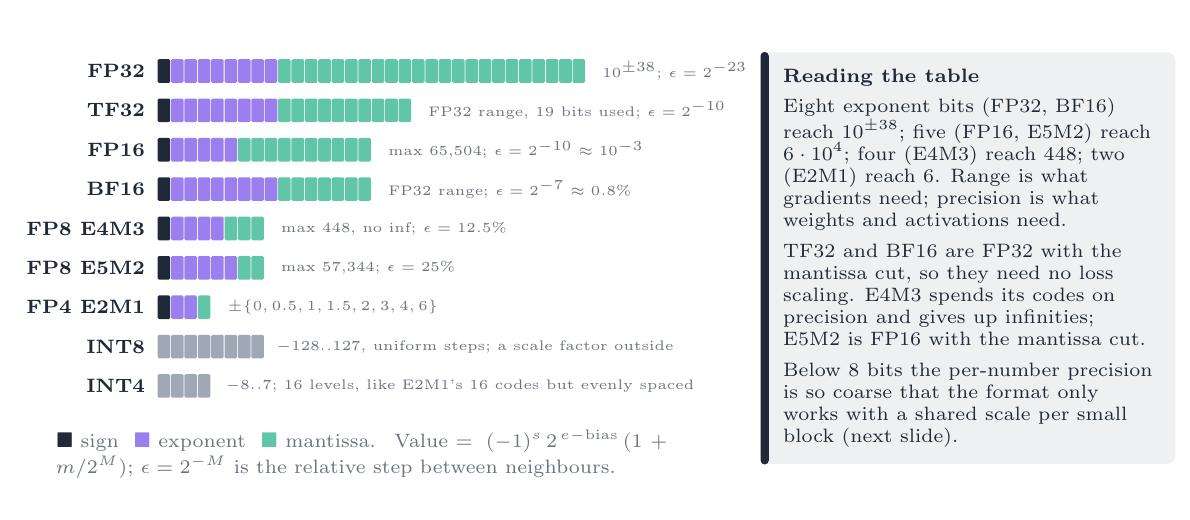
\begin{tikzpicture}
  \useasboundingbox (0,0) rectangle (14.4,5.9);
  % bit layouts: name / sign / exp / man / color scheme
  \foreach \y/\name/\e/\m/\note in {5.35/{FP32}/8/23/{$10^{\pm38}$; $\epsilon=2^{-23}$},
                                   4.85/{TF32}/8/10/{FP32 range, 19 bits used; $\epsilon=2^{-10}$},
                                   4.35/{FP16}/5/10/{max 65{,}504; $\epsilon=2^{-10}\approx10^{-3}$},
                                   3.85/{BF16}/8/7/{FP32 range; $\epsilon=2^{-7}\approx0.8\%$},
                                   3.35/{FP8 E4M3}/4/3/{max 448, no inf; $\epsilon=12.5\%$},
                                   2.85/{FP8 E5M2}/5/2/{max 57{,}344; $\epsilon=25\%$},
                                   2.35/{FP4 E2M1}/2/1/{$\pm\{0,0.5,1,1.5,2,3,4,6\}$}}{
    \node[lab,anchor=east,font=\scriptsize\bfseries,text=ink] at (1.55,\y) {\name};
    \fill[ink,rounded corners=0.5pt] (1.65,\y-0.15) rectangle ++(0.16,0.3);
    \foreach \i in {1,...,\e}{\fill[posc!70,rounded corners=0.5pt] ({1.65+\i*0.17},\y-0.15) rectangle ++(0.16,0.3);}
    \foreach \i in {1,...,\m}{\fill[emb!65,rounded corners=0.5pt] ({1.65+(\e+\i)*0.17},\y-0.15) rectangle ++(0.16,0.3);}
    \node[lab,anchor=west,font=\tiny] at ({1.75+(\e+\m+1)*0.17+0.05},\y) {\note};}
  \node[lab,anchor=east,font=\scriptsize\bfseries,text=ink] at (1.55,1.85) {INT8};
  \foreach \i in {0,...,7}{\fill[tok!60,rounded corners=0.5pt] ({1.65+\i*0.17},1.7) rectangle ++(0.16,0.3);}
  \node[lab,anchor=west,font=\tiny] at (3.1,1.85) {$-128..127$, uniform steps; a scale factor outside};
  \node[lab,anchor=east,font=\scriptsize\bfseries,text=ink] at (1.55,1.35) {INT4};
  \foreach \i in {0,...,3}{\fill[tok!60,rounded corners=0.5pt] ({1.65+\i*0.17},1.2) rectangle ++(0.16,0.3);}
  \node[lab,anchor=west,font=\tiny] at (2.45,1.35) {$-8..7$; 16 levels, like E2M1's 16 codes but evenly spaced};
  \node[lab,anchor=north west,text width=8.4cm] at (0.3,0.85) {{\color{ink}$\blacksquare$} sign \ {\color{posc!70}$\blacksquare$} exponent \ {\color{emb!65}$\blacksquare$} mantissa. \ Value $=(-1)^s\,2^{\,e-\text{bias}}\,(1+m/2^{M})$; $\epsilon=2^{-M}$ is the relative step between neighbours.};
  \bgpanels{9.3}{5.6}{4.7cm}{Reading the table}{%
    Eight exponent bits (FP32, BF16) reach $10^{\pm38}$; five (FP16, E5M2) reach
    $6\cdot10^4$; four (E4M3) reach 448; two (E2M1) reach 6. Range is what
    gradients need; precision is what weights and activations need.\\[3pt]
    TF32 and BF16 are FP32 with the mantissa cut, so they need no loss scaling.
    E4M3 spends its codes on precision and gives up infinities; E5M2 is FP16
    with the mantissa cut.\\[3pt]
    Below 8 bits the per-number precision is so coarse that the format only
    works with a shared scale per small block (next slide).}
\end{tikzpicture}
\end{frame}

% ---------------------------------------------------------------- 19
\begin{frame}{Scale factors: where the lost bits go}
\framesubtitle{A low-precision number is a code times a scale. The question is how many numbers share one scale.}
\centering
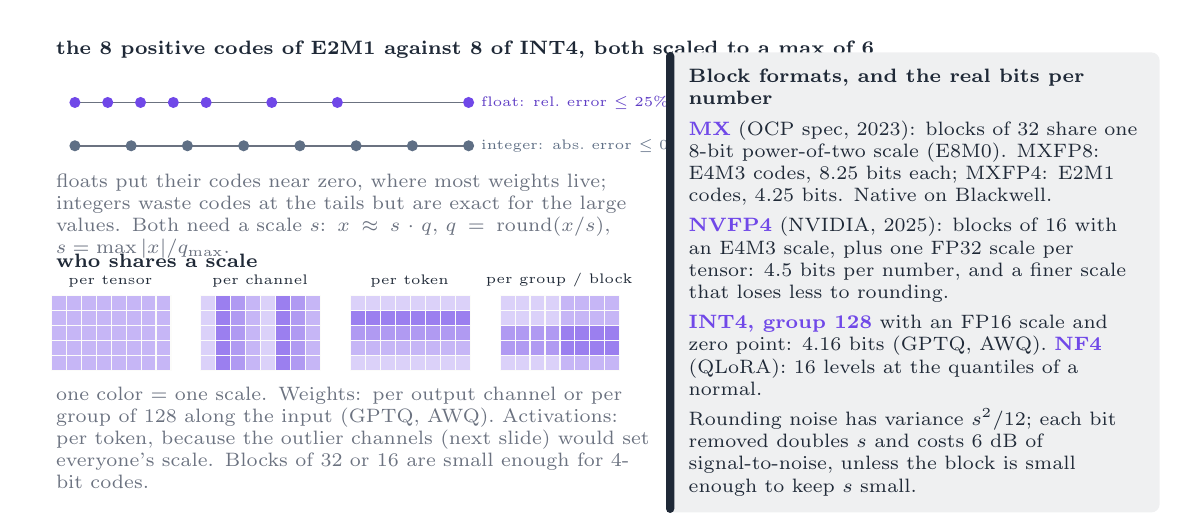
\begin{tikzpicture}
  \useasboundingbox (0,0) rectangle (14.4,5.9);
  % number lines
  \node[lab,anchor=south west,font=\scriptsize\bfseries,text=ink] at (0.3,5.45) {the 8 positive codes of E2M1 against 8 of INT4, both scaled to a max of 6};
  \draw[muted,line width=0.6pt] (0.6,4.95) -- (5.6,4.95);
  \foreach \v in {0,0.5,1,1.5,2,3,4,6}{\fill[posc] ({0.6+\v*0.8333},4.95) circle (2pt);}
  \node[lab,anchor=west,font=\tiny,text=posc!85!black] at (5.7,4.95) {float: rel.\ error $\le25\%$};
  \draw[muted,line width=0.6pt] (0.6,4.4) -- (5.6,4.4);
  \foreach \i in {0,...,7}{\fill[tok] ({0.6+\i*5/7},4.4) circle (2pt);}
  \node[lab,anchor=west,font=\tiny,text=tok] at (5.7,4.4) {integer: abs.\ error $\le0.43$};
  \node[lab,anchor=north west,text width=7.5cm] at (0.3,4.1) {floats put their codes near zero, where most weights live; integers waste codes at the tails but are exact for the large values. Both need a scale $s$: $x\approx s\cdot q$, $q=\mathrm{round}(x/s)$, $s=\max|x|/q_{\max}$.};
  % granularity diagram
  \node[lab,anchor=south west,font=\scriptsize\bfseries,text=ink] at (0.3,2.8) {who shares a scale};
  \foreach \k/\x/\ttl in {0/0.3/{per tensor},1/2.2/{per channel},2/4.1/{per token},3/6.0/{per group / block}}{
    \node[lab,anchor=south,font=\tiny,text=ink] at (\x+0.75,2.55) {\ttl};
    \foreach \r in {0,...,4}{\foreach \c in {0,...,7}{
      \ifnum\k=0 \pgfmathtruncatemacro{\sh}{40}\fi
      \ifnum\k=1 \pgfmathtruncatemacro{\sh}{25+mod(\c*3,4)*15}\fi
      \ifnum\k=2 \pgfmathtruncatemacro{\sh}{25+mod(\r*3,4)*15}\fi
      \ifnum\k=3 \pgfmathtruncatemacro{\sh}{25+mod(int(\c/4)+int(\r/2)*2,4)*15}\fi
      \fill[posc!\sh!white,draw=paper,line width=0.4pt] ({\x+\c*0.19},{2.5-\r*0.19-0.19}) rectangle ++(0.19,0.19);}}}
  \node[lab,anchor=north west,text width=7.6cm] at (0.3,1.4) {one color = one scale. Weights: per output channel or per group of 128 along the input (GPTQ, AWQ). Activations: per token, because the outlier channels (next slide) would set everyone's scale. Blocks of 32 or 16 are small enough for 4-bit codes.};
  \bgpanels{8.1}{5.6}{5.7cm}{Block formats, and the real bits per number}{%
    \hl{posc}{MX} (OCP spec, 2023): blocks of 32 share one 8-bit power-of-two
    scale (E8M0). MXFP8: E4M3 codes, 8.25 bits each; MXFP4: E2M1 codes,
    4.25 bits. Native on Blackwell.\\[3pt]
    \hl{posc}{NVFP4} (NVIDIA, 2025): blocks of 16 with an E4M3 scale, plus
    one FP32 scale per tensor: 4.5 bits per number, and a finer scale that
    loses less to rounding.\\[3pt]
    \hl{posc}{INT4, group 128} with an FP16 scale and zero point: 4.16 bits
    (GPTQ, AWQ). \hl{posc}{NF4} (QLoRA): 16 levels at the quantiles of a normal.\\[3pt]
    Rounding noise has variance $s^2/12$; each bit removed doubles $s$ and
    costs 6 dB of signal-to-noise, unless the block is small enough to keep
    $s$ small.}
\end{tikzpicture}
\end{frame}

% ---------------------------------------------------------------- 20
\begin{frame}{Outliers: the few channels that set everyone's scale}
\framesubtitle{A few hidden dimensions carry values far larger than the rest; every low-precision method works around them.}
\centering
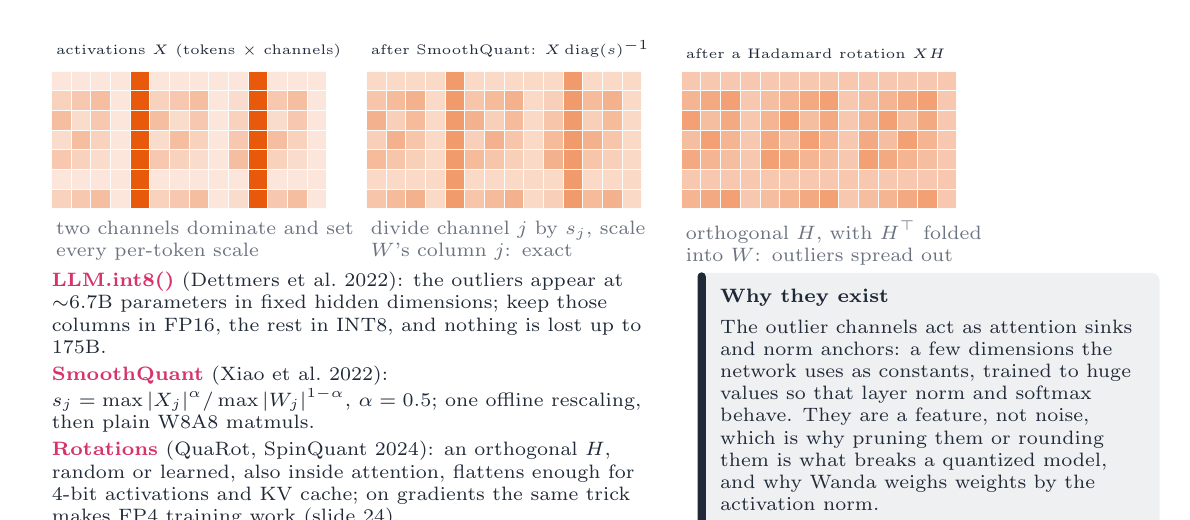
\begin{tikzpicture}
  \useasboundingbox (0,0) rectangle (14.4,5.9);
  \foreach \k/\x/\ttl in {0/0.3/{activations $X$ (tokens $\times$ channels)},1/4.3/{after SmoothQuant: $X\,\mathrm{diag}(s)^{-1}$},2/8.3/{after a Hadamard rotation $XH$}}{
    \node[lab,anchor=south west,font=\tiny,text=ink] at (\x,5.45) {\ttl};
    \foreach \r in {0,...,6}{\foreach \c in {0,...,13}{
      \pgfmathtruncatemacro{\base}{15+mod(\r*7+\c*5+\r*\c,5)*6}
      \ifnum\k=0 \pgfmathtruncatemacro{\sh}{ifthenelse(\c==4||\c==10,100,\base)}\fi
      \ifnum\k=1 \pgfmathtruncatemacro{\sh}{ifthenelse(\c==4||\c==10,60,\base+8)}\fi
      \ifnum\k=2 \pgfmathtruncatemacro{\sh}{\base+18}\fi
      \fill[attn!\sh!white,draw=paper,line width=0.3pt] ({\x+\c*0.25},{5.1-\r*0.25}) rectangle ++(0.25,0.25);}}}
  \node[lab,anchor=north west,text width=3.8cm] at (0.3,3.5) {two channels dominate and set every per-token scale};
  \node[lab,anchor=north west,text width=3.8cm] at (4.3,3.5) {divide channel $j$ by $s_j$, scale $W$'s column $j$: exact};
  \node[lab,anchor=north west,text width=3.8cm] at (8.3,3.5) {orthogonal $H$, with $H^\top$ folded into $W$: outliers spread out};
  \node[txt,anchor=north west,text width=7.9cm,font=\scriptsize] at (0.3,2.8) {%
    \hl{outc}{LLM.int8()} (Dettmers et al.\ 2022): the outliers appear at
    $\sim$6.7B parameters in fixed hidden dimensions; keep those columns in
    FP16, the rest in INT8, and nothing is lost up to 175B.\\[2pt]
    \hl{outc}{SmoothQuant} (Xiao et al.\ 2022): $s_j=\max|X_j|^{\alpha}/\max|W_j|^{1-\alpha}$,
    $\alpha=0.5$; one offline rescaling, then plain W8A8 matmuls.\\[2pt]
    \hl{outc}{Rotations} (QuaRot, SpinQuant 2024): an orthogonal $H$, random or
    learned, also inside attention, flattens enough for 4-bit activations and
    KV cache; on gradients the same trick makes FP4 training work (slide 24).};
  \bgpanels{8.5}{2.8}{5.3cm}{Why they exist}{%
    The outlier channels act as attention sinks and norm anchors: a few
    dimensions the network uses as constants, trained to huge values so
    that layer norm and softmax behave. They are a feature, not noise,
    which is why pruning them or rounding them is what breaks a quantized
    model, and why Wanda weighs weights by the activation norm.}
\end{tikzpicture}
\end{frame}

% ---------------------------------------------------------------- 21
\begin{frame}{What the tensor cores run, by generation}
\framesubtitle{Each generation halves the smallest native format and doubles its throughput; bandwidth grows slower than FLOPs.}
\centering
\begin{tikzpicture}
  \useasboundingbox (0,0) rectangle (14.4,5.9);
  \node[anchor=north west,inner sep=0,font=\fontsize{6.3}{7.6}\selectfont] at (0.2,5.75) {%
    \renewcommand{\arraystretch}{1.2}\setlength{\tabcolsep}{3.5pt}%
    \begin{tabular}{@{}llrrrrrr@{}}
      \toprule
      \textbf{GPU (year)} & \textbf{new native formats} & \textbf{BF16} & \textbf{FP8} & \textbf{FP4} & \textbf{HBM} & \textbf{bandwidth} & \textbf{ridge (BF16)}\\
      & & \multicolumn{3}{c}{dense tensor TFLOP/s} & GB & TB/s & FLOP/byte\\
      \midrule
      A100 (2020) & TF32, BF16, INT8; 2:4 sparsity & 312 & -- & -- & 80 & 2.0 & 156\\
      H100 SXM (2022) & FP8 E4M3/E5M2 (Transformer Engine) & 989 & 1,979 & -- & 80 & 3.35 & 295\\
      B200 (2024) & FP4 (NVFP4, MXFP4), FP6; 2nd-gen TE & 2,250 & 4,500 & 9,000 & 180 & 8.0 & 281\\
      MI300X (2023) & FP8 & 1,307 & 2,615 & -- & 192 & 5.3 & 247\\
      MI355X (2025) & FP4, FP6 & 2,520 & 5,030 & 10,070 & 288 & 8.0 & 315\\
      Rubin (2026)$^\dagger$ & NVFP4 training at 35 PFLOP/s, HBM4 & -- & -- & 35,000 & 288 & 22 & --\\
      \bottomrule
    \end{tabular}};
  \node[lab,anchor=north west,text width=13.8cm] at (0.3,2.6) {vendor datasheet peaks, dense (headline numbers are usually ``with sparsity'', twice these); B200 per GPU is derived from the 8-GPU HGX totals; Rubin from NVIDIA's 2026 announcement. Ridge $=$ BF16 peak over bandwidth, derived. Decode at batch 1 sits at 1--4 FLOP/byte on all of them.};
  \foreach \x/\c/\ttl/\body in {
      0.2/posc/{Format support is the lever}/{A format pays only when the tensor core runs it natively: INT8 on Ampere, FP8 on Hopper, FP4 on Blackwell. Each moved the serving default.},
      4.95/posc/{FLOPs outrun bytes}/{A100 to B200: dense BF16 up 7$\times$, bandwidth 4$\times$. Decode gets more memory-bound every generation; the case for fewer bits grows with it.},
      9.7/posc/{Accumulation is the fine print}/{Products are summed in a wider accumulator; how wide matters. DeepSeek-V3 measured $\sim$14 bits on H800's FP8 path and moved partials to FP32 every 128 terms.}}{
    \node[anchor=north west,inner sep=0] at (\x,1.95) {%
      \begin{tikzpicture}
        \node[anchor=north west,text width=4.25cm,align=flush left,font=\scriptsize,text=ink,minimum height=1.85cm,
              inner xsep=6pt,inner ysep=4pt,rounded corners=3pt,fill=\c!8] (c)
              {{\color{\c}\bfseries\ttl}\\[2pt]\body};
      \end{tikzpicture}};}
\end{tikzpicture}
\end{frame}

% ---------------------------------------------------------------- 22
\stage{6}
\begin{frame}{Mixed-precision training: master weights, loss scaling, BF16}
\framesubtitle{Compute in 16 bits, accumulate and update in 32: the recipe since 2017, and why BF16 made it simpler.}
\centering
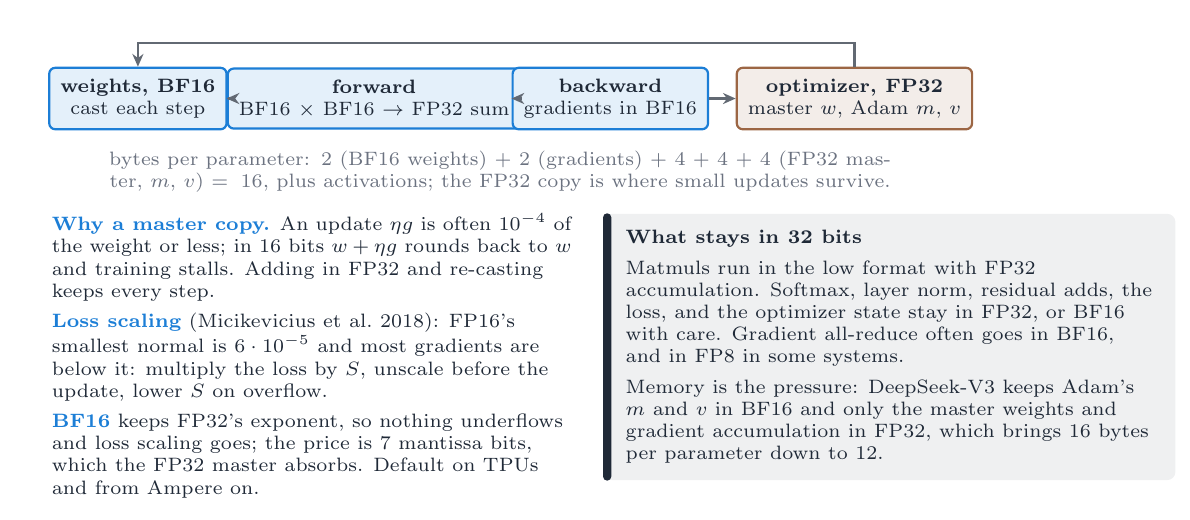
\begin{tikzpicture}
  \useasboundingbox (0,0) rectangle (14.4,5.9);
  \node[comp=mlp,minimum width=2.2cm,minimum height=0.75cm,font=\scriptsize,align=center] (w16) at (1.4,5.0) {\textbf{weights, BF16}\\cast each step};
  \node[comp=mlp,minimum width=2.2cm,minimum height=0.75cm,font=\scriptsize,align=center] (fwd) at (4.4,5.0) {\textbf{forward}\\BF16 $\times$ BF16 $\to$ FP32 sum};
  \node[comp=mlp,minimum width=2.2cm,minimum height=0.75cm,font=\scriptsize,align=center] (bwd) at (7.4,5.0) {\textbf{backward}\\gradients in BF16};
  \node[comp=trn,minimum width=2.4cm,minimum height=0.75cm,font=\scriptsize,align=center] (opt) at (10.5,5.0) {\textbf{optimizer, FP32}\\master $w$, Adam $m$, $v$};
  \draw[flow] (w16) -- (fwd); \draw[flow] (fwd) -- (bwd); \draw[flow] (bwd) -- (opt);
  \draw[flow] (opt.north) -- ++(0,0.3) -| (w16.north);
  \node[lab,anchor=north,text width=11cm,align=center] at (6.0,4.4) {bytes per parameter: 2 (BF16 weights) + 2 (gradients) + 4 + 4 + 4 (FP32 master, $m$, $v$) $=16$, plus activations; the FP32 copy is where small updates survive.};
  \node[txt,anchor=north west,text width=6.6cm,font=\scriptsize] at (0.3,3.55) {%
    \hl{mlp}{Why a master copy.} An update $\eta g$ is often $10^{-4}$ of the
    weight or less; in 16 bits $w+\eta g$ rounds back to $w$ and training
    stalls. Adding in FP32 and re-casting keeps every step.\\[3pt]
    \hl{mlp}{Loss scaling} (Micikevicius et al.\ 2018): FP16's smallest normal is
    $6\cdot10^{-5}$ and most gradients are below it: multiply the loss by $S$,
    unscale before the update, lower $S$ on overflow.\\[3pt]
    \hl{mlp}{BF16} keeps FP32's exponent, so nothing underflows and loss
    scaling goes; the price is 7 mantissa bits, which the FP32 master
    absorbs. Default on TPUs and from Ampere on.};
  \bgpanels{7.3}{3.55}{6.7cm}{What stays in 32 bits}{%
    Matmuls run in the low format with FP32 accumulation. Softmax, layer
    norm, residual adds, the loss, and the optimizer state stay in FP32,
    or BF16 with care. Gradient all-reduce often goes in BF16, and in FP8 in
    some systems.\\[3pt]
    Memory is the pressure: DeepSeek-V3 keeps Adam's $m$ and $v$ in BF16
    and only the master weights and gradient accumulation in FP32, which
    brings 16 bytes per parameter down to 12.}
\end{tikzpicture}
\end{frame}

% ---------------------------------------------------------------- 23
\begin{frame}{FP8 training: the scale goes per tensor, then per tile}
\framesubtitle{Eight bits hold a GEMM if each small block has its own scale and the sums are carried in 32.}
\centering
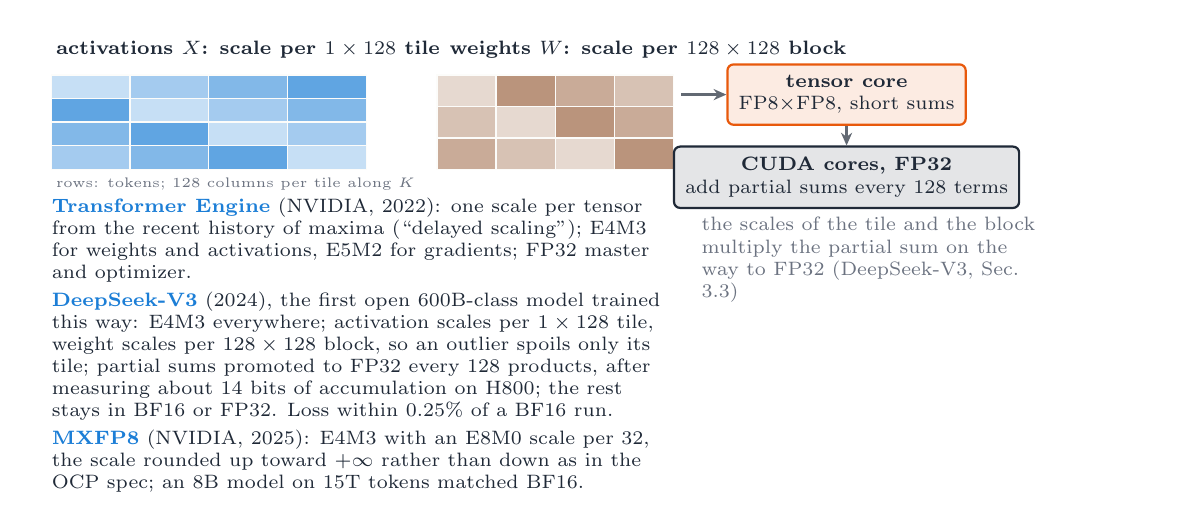
\begin{tikzpicture}
  \useasboundingbox (0,0) rectangle (14.4,5.9);
  % X tiles (1 x 128) and W blocks (128 x 128)
  \node[lab,anchor=south west,font=\scriptsize\bfseries,text=ink] at (0.3,5.45) {activations $X$: scale per $1\times128$ tile};
  \foreach \r in {0,...,3}{\foreach \c in {0,...,3}{
    \pgfmathtruncatemacro{\sh}{25+mod(\r*3+\c*5,4)*15}
    \fill[mlp!\sh!white,draw=paper,line width=0.5pt] ({0.3+\c*1.0},{5.0-\r*0.3}) rectangle ++(1.0,0.3);}}
  \node[lab,anchor=north west,font=\tiny] at (0.3,4.05) {rows: tokens; 128 columns per tile along $K$};
  \node[lab,anchor=south west,font=\scriptsize\bfseries,text=ink] at (5.3,5.45) {weights $W$: scale per $128\times128$ block};
  \foreach \r in {0,...,2}{\foreach \c in {0,...,3}{
    \pgfmathtruncatemacro{\sh}{25+mod(\r*5+\c*3,4)*15}
    \fill[trn!\sh!white,draw=paper,line width=0.5pt] ({5.2+\c*0.75},{4.9-\r*0.4}) rectangle ++(0.75,0.4);}}
  \node[comp=attn,minimum width=2.4cm,minimum height=0.6cm,font=\scriptsize,align=center] (tc) at (10.4,5.05) {\textbf{tensor core}\\FP8$\times$FP8, short sums};
  \node[comp=ink,minimum width=2.4cm,minimum height=0.6cm,font=\scriptsize,align=center] (cc) at (10.4,4.0) {\textbf{CUDA cores, FP32}\\add partial sums every 128 terms};
  \draw[flow] (8.3,5.05) -- (tc); \draw[flow] (tc) -- (cc);
  \node[lab,anchor=north west,text width=4.4cm] at (8.5,3.55) {the scales of the tile and the block multiply the partial sum on the way to FP32 (DeepSeek-V3, Sec.\ 3.3)};
  \node[txt,anchor=north west,text width=7.9cm,font=\scriptsize] at (0.3,3.75) {%
    \hl{mlp}{Transformer Engine} (NVIDIA, 2022): one scale per tensor from the
    recent history of maxima (``delayed scaling''); E4M3 for weights and
    activations, E5M2 for gradients; FP32 master and optimizer.\\[2pt]
    \hl{mlp}{DeepSeek-V3} (2024), the first open 600B-class model trained
    this way: E4M3 everywhere; activation scales per $1\times128$ tile, weight
    scales per $128\times128$ block, so an outlier spoils only its tile;
    partial sums promoted to FP32 every 128 products, after measuring
    about 14 bits of accumulation on H800; the rest stays in BF16 or FP32.
    Loss within 0.25\% of a BF16 run.\\[2pt]
    \hl{mlp}{MXFP8} (NVIDIA, 2025): E4M3 with an E8M0 scale per 32, the scale
    rounded up toward $+\infty$ rather than down as in the OCP spec; an 8B
    model on 15T tokens matched BF16.};
\end{tikzpicture}
\end{frame}

% ---------------------------------------------------------------- 24
\begin{frame}{FP4 training arrives}
\framesubtitle{Four bits need everything the FP8 recipe has, plus unbiased rounding and a rotation before quantizing.}
\centering
\begin{tikzpicture}
  \useasboundingbox (0,0) rectangle (14.4,5.9);
  \chev{0.2}{5.1}{2.0}{tok}{FP32}
  \chev{2.25}{5.1}{3.1}{mlp!70}{FP16 + loss scaling}
  \chev{5.4}{5.1}{2.0}{mlp!85}{BF16}
  \chev{7.45}{5.1}{2.7}{mlp}{FP8}
  \chev{10.2}{5.1}{3.6}{posc}{FP4: MXFP4, NVFP4}
  \foreach \x/\t in {1.2/{2012},3.8/{2017},6.4/{2019--20},8.8/{2022: TE; 2024: DeepSeek-V3},12.0/{2025}}{\node[lab,anchor=north,font=\tiny] at (\x,5.05) {\t};}
  \node[lab,anchor=north west,text width=13.8cm] at (0.3,4.7) {each step halves the matmul input bits and doubles throughput; each needed a new trick to keep the gradients.};
  \foreach \x/\y/\c/\ttl/\body in {
      0.2/4.25/posc/{2D block scaling for weights}/{a $16\times16$ block shares its scale, so $W$ and $W^\top$ quantize identically in the forward and backward passes.},
      4.95/4.25/posc/{Random Hadamard transforms}/{rotate gradients (and activations) before quantizing so no single outlier sets a block's scale; undone exactly after the matmul.},
      9.7/4.25/posc/{Stochastic rounding}/{round up or down with probability given by the remainder: unbiased gradients, where round-to-nearest pushes small updates to zero.},
      0.2/2.25/posc/{Keep the sensitive layers}/{embeddings, norms, the output head and the first and last blocks stay in BF16 or FP8; NVFP4 pretraining kept 16\% of the linear layers higher.},
      4.95/2.25/posc/{What was shown}/{NVFP4 (NVIDIA 2025): 12B on 10T tokens, loss gap 1--1.5\% vs FP8, tasks matched$^\ast$. MXFP4 (Tseng 2025): near-lossless with SR + RHT.},
      9.7/2.25/posc/{Where it stands}/{Nemotron 3 Ultra (June 2026): 550B/55B pretrained in NVFP4 on 20T tokens, loss gap under 0.4\%$^\dagger$. DeepSeek-V4 ships expert weights in FP4$^\dagger$.}}{
    \node[anchor=north west,inner sep=0] at (\x,\y) {%
      \begin{tikzpicture}
        \node[anchor=north west,text width=4.25cm,align=flush left,font=\scriptsize,text=ink,minimum height=1.85cm,
              inner xsep=6pt,inner ysep=4pt,rounded corners=3pt,fill=\c!8] (c)
              {{\color{\c}\bfseries\ttl}\\[2pt]\body};
      \end{tikzpicture}};}
  \node[lab,anchor=north west,text width=13.8cm,font=\tiny] at (0.3,0.3) {$^\ast$numbers as reported by the authors; $^\dagger$from vendor and lab write-ups, see the sources slide.};
\end{tikzpicture}
\end{frame}

% ---------------------------------------------------------------- 25
\stage{7}
\begin{frame}{Scaling laws for precision}
\framesubtitle{Bits are a resource like parameters and tokens: there is a compute-optimal precision, and it is not 16.}
\centering
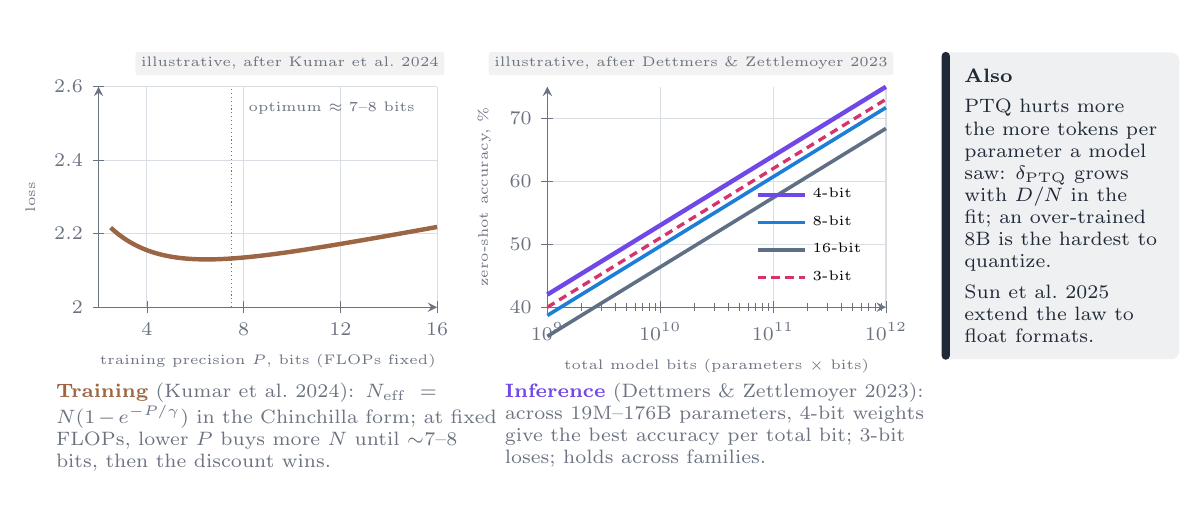
\begin{tikzpicture}
  \useasboundingbox (0,0) rectangle (14.4,5.9);
  \begin{axis}[lecture,at={(0.9cm,2.35cm)},anchor=south west,scale only axis,width=4.3cm,height=2.8cm,
      xmin=2,xmax=16,ymin=2.0,ymax=2.6,domain=2.5:16,samples=80,xtick={4,8,12,16},ytick={2.0,2.2,2.4,2.6},
      xlabel={training precision $P$, bits (FLOPs fixed)},ylabel={loss},x label style={font=\tiny},y label style={font=\tiny}]
    \addplot[trn,line width=1.6pt] {2.05+0.5*exp(-x/2.2)+0.012*(x-2)};
    \draw[muted,densely dotted] (axis cs:7.5,2.0) -- (axis cs:7.5,2.6);
    \node[font=\tiny,text=muted,anchor=south west] at (axis cs:7.8,2.5) {optimum $\approx7$--8 bits};
  \end{axis}
  \srctag{5.3}{5.6}{illustrative, after Kumar et al.\ 2024}
  \begin{axis}[lecture,at={(6.6cm,2.35cm)},anchor=south west,scale only axis,width=4.3cm,height=2.8cm,
      xmode=log,xmin=1e9,xmax=1e12,ymin=40,ymax=75,domain=1e9:1e12,samples=60,xtick={1e9,1e10,1e11,1e12},ytick={40,50,60,70},
      xlabel={total model bits (parameters $\times$ bits)},ylabel={zero-shot accuracy, \%},x label style={font=\tiny},y label style={font=\tiny},
      legend style={font=\tiny,at={(0.97,0.05)},anchor=south east}]
    \addplot[posc,line width=1.6pt] {42+11*(ln(x/1e9)/ln(10))}; \addlegendentry{4-bit}
    \addplot[mlp,line width=1.3pt] {42+11*(ln(x/2e9)/ln(10))}; \addlegendentry{8-bit}
    \addplot[tok,line width=1.3pt] {42+11*(ln(x/4e9)/ln(10))}; \addlegendentry{16-bit}
    \addplot[outc,densely dashed,line width=1.2pt] {40+11*(ln(x/1e9)/ln(10))}; \addlegendentry{3-bit}
  \end{axis}
  \srctag{11.0}{5.6}{illustrative, after Dettmers \& Zettlemoyer 2023}
  \node[lab,anchor=north west,text width=5.6cm] at (0.3,1.45) {\hl{trn}{Training} (Kumar et al.\ 2024): $N_{\text{eff}}=N(1-e^{-P/\gamma})$ in the Chinchilla form; at fixed FLOPs, lower $P$ buys more $N$ until $\sim$7--8 bits, then the discount wins.};
  \node[lab,anchor=north west,text width=5.6cm] at (6.0,1.45) {\hl{posc}{Inference} (Dettmers \& Zettlemoyer 2023): across 19M--176B parameters, 4-bit weights give the best accuracy per total bit; 3-bit loses; holds across families.};
  \bgpanels{11.6}{5.6}{2.45cm}{Also}{%
    PTQ hurts more the more tokens per parameter a model saw:
    $\delta_{\text{PTQ}}$ grows with $D/N$ in the fit; an over-trained 8B is
    the hardest to quantize.\\[3pt]
    Sun et al.\ 2025 extend the law to float formats.}
\end{tikzpicture}
\end{frame}

% ---------------------------------------------------------------- 26
\stage{8}
\begin{frame}{Post-training quantization I: weights only}
\framesubtitle{Round the weights to 4 bits after training, one layer at a time; decode gets faster because it reads fewer bytes.}
\centering
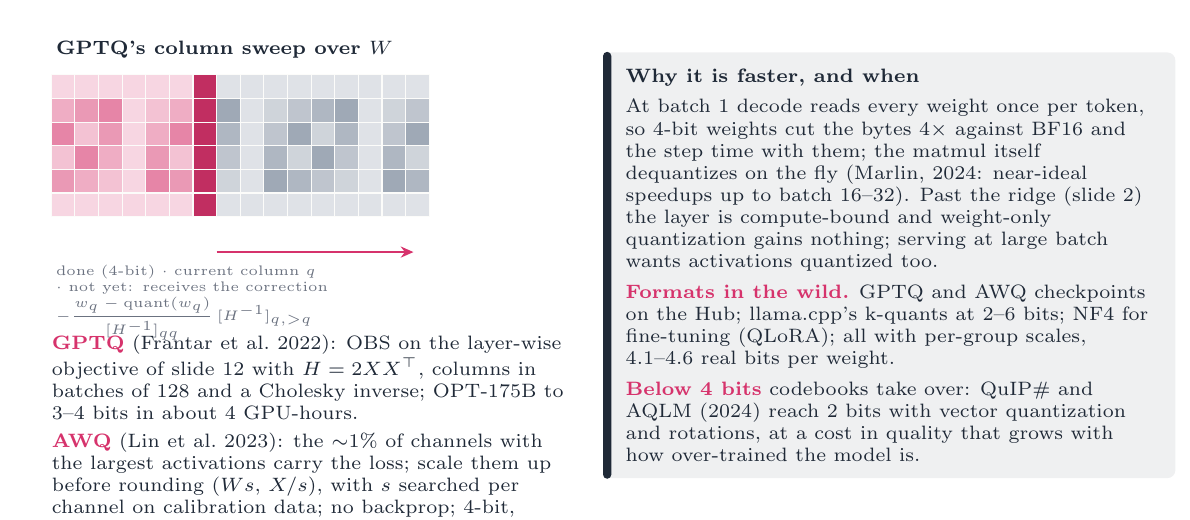
\begin{tikzpicture}
  \useasboundingbox (0,0) rectangle (14.4,5.9);
  % GPTQ column sweep
  \node[lab,anchor=south west,font=\scriptsize\bfseries,text=ink] at (0.3,5.45) {GPTQ's column sweep over $W$};
  \foreach \r in {0,...,5}{\foreach \c in {0,...,15}{
    \pgfmathtruncatemacro{\sh}{20+mod(\r*7+\c*5+\r*\c,5)*10}
    \ifnum\c<6 \fill[outc!\sh!white,draw=paper,line width=0.4pt] ({0.3+\c*0.3},{5.0-\r*0.3}) rectangle ++(0.3,0.3);
    \else \ifnum\c=6 \fill[outc!90!black,draw=paper,line width=0.4pt] ({0.3+\c*0.3},{5.0-\r*0.3}) rectangle ++(0.3,0.3);
    \else \fill[tok!\sh!white,draw=paper,line width=0.4pt] ({0.3+\c*0.3},{5.0-\r*0.3}) rectangle ++(0.3,0.3); \fi\fi}}
  \draw[flow,outc] (2.4,3.05) -- (4.9,3.05);
  \node[lab,anchor=north west,font=\tiny,text width=4.8cm] at (0.3,2.95) {done (4-bit) $\cdot$ current column $q$ $\cdot$ not yet: receives the correction $-\dfrac{w_q-\mathrm{quant}(w_q)}{[H^{-1}]_{qq}}\,[H^{-1}]_{q,>q}$};
  \node[txt,anchor=north west,text width=6.5cm,font=\scriptsize] at (0.3,2.0) {%
    \hl{outc}{GPTQ} (Frantar et al.\ 2022): OBS on the layer-wise objective of
    slide 12 with $H=2XX^\top$, columns in batches of 128 and a Cholesky
    inverse; OPT-175B to 3--4 bits in about 4 GPU-hours.\\[2pt]
    \hl{outc}{AWQ} (Lin et al.\ 2023): the $\sim$1\% of channels with the
    largest activations carry the loss; scale them up before rounding
    ($Ws$, $X/s$), with $s$ searched per channel on calibration data; no
    backprop; 4-bit, groups of 128.};
  \bgpanels{7.3}{5.6}{6.7cm}{Why it is faster, and when}{%
    At batch 1 decode reads every weight once per token, so 4-bit weights
    cut the bytes 4$\times$ against BF16 and the step time with them; the
    matmul itself dequantizes on the fly (Marlin, 2024: near-ideal
    speedups up to batch 16--32). Past the ridge (slide 2) the layer is
    compute-bound and weight-only quantization gains nothing; serving at
    large batch wants activations quantized too.\\[3pt]
    \hl{outc}{Formats in the wild.} GPTQ and AWQ checkpoints on the Hub;
    llama.cpp's k-quants at 2--6 bits; NF4 for fine-tuning (QLoRA);
    all with per-group scales, 4.1--4.6 real bits per weight.\\[3pt]
    \hl{outc}{Below 4 bits} codebooks take over: QuIP\# and AQLM (2024)
    reach 2 bits with vector quantization and rotations, at a cost in
    quality that grows with how over-trained the model is.}
\end{tikzpicture}
\end{frame}

% ---------------------------------------------------------------- 27
\begin{frame}{Post-training quantization II: activations too}
\framesubtitle{Weight bits help decode; activation bits help prefill and large batches. Hardware decides which pairs run natively.}
\centering
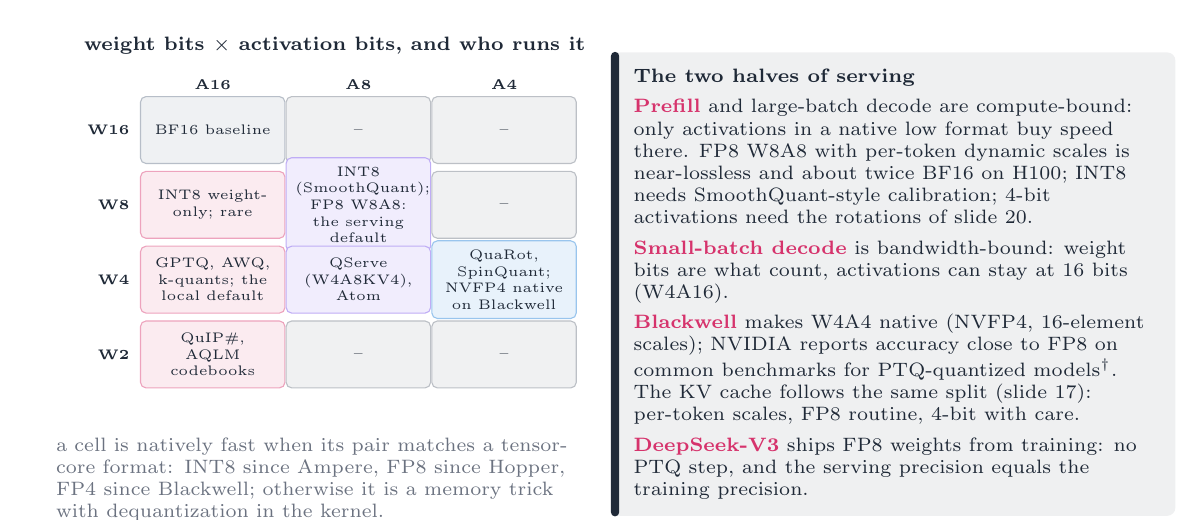
\begin{tikzpicture}
  \useasboundingbox (0,0) rectangle (14.4,5.9);
  % W x A grid
  \node[lab,anchor=south,font=\scriptsize\bfseries,text=ink] at (3.9,5.5) {weight bits $\times$ activation bits, and who runs it};
  \foreach \j/\alab in {0/{A16},1/{A8},2/{A4}}{\node[lab,anchor=south,font=\tiny\bfseries,text=ink] at ({2.35+\j*1.85},5.05) {\alab};}
  \foreach \i/\wlab in {0/{W16},1/{W8},2/{W4},3/{W2}}{\node[lab,anchor=east,font=\tiny\bfseries,text=ink] at (1.35,{4.6-\i*0.95}) {\wlab};}
  \foreach \i/\j/\c/\t in {0/0/tok/{BF16 baseline},
                          1/0/outc/{INT8 weight-only; rare},
                          2/0/outc/{GPTQ, AWQ, k-quants; the local default},
                          3/0/outc/{QuIP\#, AQLM codebooks},
                          0/1/muted/{--},
                          1/1/posc/{INT8 (SmoothQuant); FP8 W8A8: the serving default},
                          2/1/posc/{QServe (W4A8KV4), Atom},
                          3/1/muted/{--},
                          0/2/muted/{--},
                          1/2/muted/{--},
                          2/2/mlp/{QuaRot, SpinQuant; NVFP4 native on Blackwell},
                          3/2/muted/{--}}{
    \node[anchor=center,text width=1.6cm,align=center,font=\tiny,text=ink,minimum height=0.85cm,minimum width=1.75cm,
          rounded corners=2pt,fill=\c!10,draw=\c!45,line width=0.4pt] at ({2.35+\j*1.85},{4.6-\i*0.95}) {\t};}
  \node[lab,anchor=north west,text width=6.5cm] at (0.3,0.75) {a cell is natively fast when its pair matches a tensor-core format: INT8 since Ampere, FP8 since Hopper, FP4 since Blackwell; otherwise it is a memory trick with dequantization in the kernel.};
  \bgpanels{7.4}{5.6}{6.6cm}{The two halves of serving}{%
    \hl{outc}{Prefill} and large-batch decode are compute-bound: only
    activations in a native low format buy speed there. FP8 W8A8 with
    per-token dynamic scales is near-lossless and about twice BF16 on
    H100; INT8 needs SmoothQuant-style calibration; 4-bit activations need
    the rotations of slide 20.\\[3pt]
    \hl{outc}{Small-batch decode} is bandwidth-bound: weight bits are what
    count, activations can stay at 16 bits (W4A16).\\[3pt]
    \hl{outc}{Blackwell} makes W4A4 native (NVFP4, 16-element scales);
    NVIDIA reports accuracy close to FP8 on common benchmarks for
    PTQ-quantized models$^\dagger$. The KV cache follows the same split
    (slide 17): per-token scales, FP8 routine, 4-bit with care.\\[3pt]
    \hl{outc}{DeepSeek-V3} ships FP8 weights from training: no PTQ step,
    and the serving precision equals the training precision.}
\end{tikzpicture}
\end{frame}

% ---------------------------------------------------------------- 28
\begin{frame}{QAT, ternary weights, and quantized experts}
\framesubtitle{When post-training rounding is not enough, train with the rounding in the loop.}
\centering
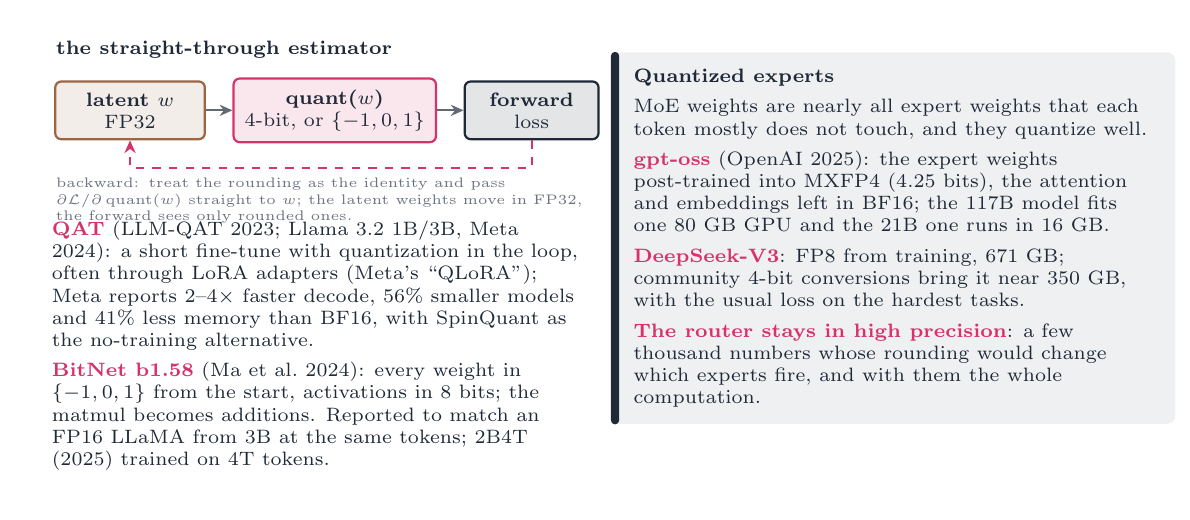
\begin{tikzpicture}
  \useasboundingbox (0,0) rectangle (14.4,5.9);
  % STE diagram
  \node[lab,anchor=south west,font=\scriptsize\bfseries,text=ink] at (0.3,5.45) {the straight-through estimator};
  \node[comp=trn,minimum width=1.9cm,minimum height=0.65cm,font=\scriptsize,align=center] (lat) at (1.3,4.85) {\textbf{latent $w$}\\FP32};
  \node[comp=outc,minimum width=1.9cm,minimum height=0.65cm,font=\scriptsize,align=center] (qz) at (3.9,4.85) {\textbf{quant($w$)}\\4-bit, or $\{-1,0,1\}$};
  \node[comp=ink,minimum width=1.7cm,minimum height=0.65cm,font=\scriptsize,align=center] (fw) at (6.4,4.85) {\textbf{forward}\\loss};
  \draw[flow] (lat) -- (qz); \draw[flow] (qz) -- (fw);
  \draw[flow,outc,dashed] (fw.south) -- ++(0,-0.35) -| (lat.south);
  \node[lab,anchor=north west,text width=6.9cm,font=\tiny] at (0.3,4.05) {backward: treat the rounding as the identity and pass $\partial\mathcal{L}/\partial\,\mathrm{quant}(w)$ straight to $w$; the latent weights move in FP32, the forward sees only rounded ones.};
  \node[txt,anchor=north west,text width=6.7cm,font=\scriptsize] at (0.3,3.45) {%
    \hl{outc}{QAT} (LLM-QAT 2023; Llama 3.2 1B/3B, Meta 2024): a short
    fine-tune with quantization in the loop, often through LoRA adapters
    (Meta's ``QLoRA''); Meta reports 2--4$\times$ faster decode, 56\% smaller
    models and 41\% less memory than BF16, with SpinQuant as the no-training
    alternative.\\[3pt]
    \hl{outc}{BitNet b1.58} (Ma et al.\ 2024): every weight in $\{-1,0,1\}$
    from the start, activations in 8 bits; the matmul becomes additions.
    Reported to match an FP16 LLaMA from 3B at the same tokens; 2B4T (2025)
    trained on 4T tokens.};
  \bgpanels{7.4}{5.6}{6.6cm}{Quantized experts}{%
    MoE weights are nearly all expert weights that each token mostly does
    not touch, and they quantize well.\\[3pt]
    \hl{outc}{gpt-oss} (OpenAI 2025): the expert weights post-trained into
    MXFP4 (4.25 bits), the attention and embeddings left in BF16; the 117B
    model fits one 80 GB GPU and the 21B one runs in 16 GB.\\[3pt]
    \hl{outc}{DeepSeek-V3}: FP8 from training, 671 GB; community 4-bit
    conversions bring it near 350 GB, with the usual loss on the hardest
    tasks.\\[3pt]
    \hl{outc}{The router stays in high precision}: a few thousand numbers
    whose rounding would change which experts fire, and with them the
    whole computation.}
\end{tikzpicture}
\end{frame}

% ---------------------------------------------------------------- 29
\begin{frame}{Measuring the damage}
\framesubtitle{Perplexity is the wrong instrument for a 4-bit model; the losses show up in long generations and hard tasks.}
\centering
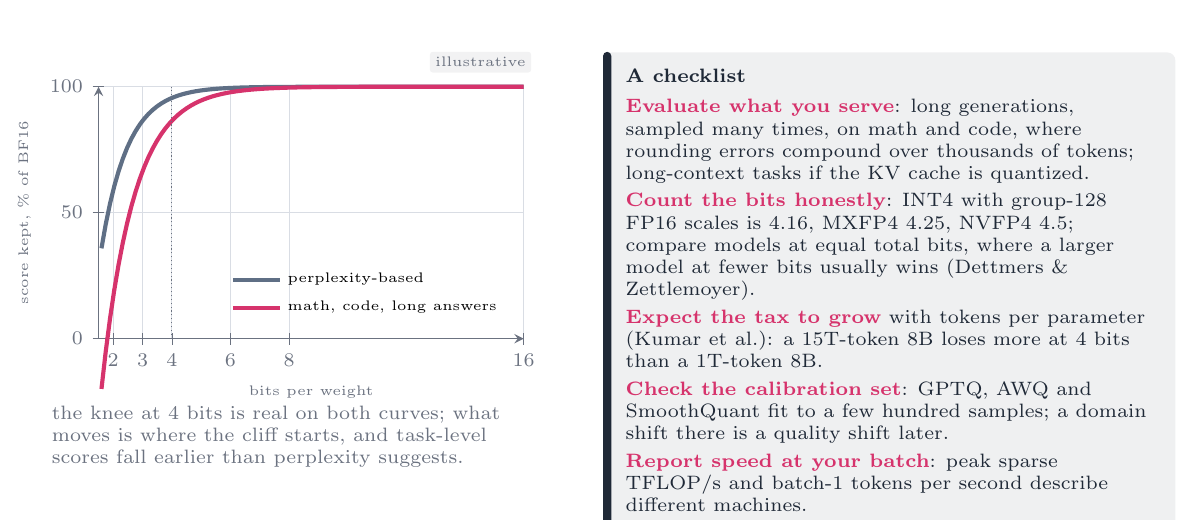
\begin{tikzpicture}
  \useasboundingbox (0,0) rectangle (14.4,5.9);
  \begin{axis}[lecture,at={(0.9cm,1.95cm)},anchor=south west,scale only axis,width=5.4cm,height=3.2cm,
      xmin=1.5,xmax=16,ymin=0,ymax=100,domain=1.6:16,samples=100,xtick={2,3,4,6,8,16},ytick={0,50,100},
      xlabel={bits per weight},ylabel={score kept, \% of BF16},x label style={font=\tiny},y label style={font=\tiny},
      legend style={font=\tiny,at={(0.97,0.05)},anchor=south east}]
    \addplot[tok,line width=1.5pt] {100-100*exp(-(x-1.2)/0.9)}; \addlegendentry{perplexity-based}
    \addplot[outc,line width=1.5pt] {100-100*exp(-(x-1.8)/1.1)}; \addlegendentry{math, code, long answers}
    \draw[muted,densely dotted] (axis cs:4,0) -- (axis cs:4,100);
  \end{axis}
  \srctag{6.4}{5.6}{illustrative}
  \node[txt,anchor=north west,text width=6.3cm,font=\scriptsize,text=muted] at (0.3,1.1)
    {the knee at 4 bits is real on both curves; what moves is where the cliff starts, and task-level scores fall earlier than perplexity suggests.};
  \bgpanels{7.3}{5.6}{6.7cm}{A checklist}{%
    \hl{outc}{Evaluate what you serve}: long generations, sampled many times, on
    math and code, where rounding errors compound over thousands of tokens;
    long-context tasks if the KV cache is quantized.\\[2pt]
    \hl{outc}{Count the bits honestly}: INT4 with group-128 FP16 scales is
    4.16, MXFP4 4.25, NVFP4 4.5; compare models at equal total bits, where a
    larger model at fewer bits usually wins (Dettmers \& Zettlemoyer).\\[2pt]
    \hl{outc}{Expect the tax to grow} with tokens per parameter (Kumar et al.):
    a 15T-token 8B loses more at 4 bits than a 1T-token 8B.\\[2pt]
    \hl{outc}{Check the calibration set}: GPTQ, AWQ and SmoothQuant fit to a
    few hundred samples; a domain shift there is a quality shift later.\\[2pt]
    \hl{outc}{Report speed at your batch}: peak sparse TFLOP/s and batch-1
    tokens per second describe different machines.}
\end{tikzpicture}
\end{frame}

% ---------------------------------------------------------------- 30
\stage{9}
\begin{frame}{Serving three models: the bill, with every lever applied}
\framesubtitle{A dense 405B, a sparse 671B and a sparse-and-quantized 117B, as they ship.}
\centering
\begin{tikzpicture}
  \useasboundingbox (0,0) rectangle (14.4,5.9);
  \node[anchor=north west,inner sep=0,font=\fontsize{6.3}{7.6}\selectfont] at (0.2,5.75) {%
    \renewcommand{\arraystretch}{1.2}\setlength{\tabcolsep}{3.5pt}%
    \begin{tabular}{@{}lrrrrrr@{}}
      \toprule
      \textbf{model} & \textbf{total / active} & \textbf{weights as shipped} & \textbf{weight bytes} & \textbf{80 GB GPUs} & \textbf{bytes per token, batch 1} & \textbf{KV per token}\\
      \midrule
      Llama 3.1 405B & 405B / 405B & BF16 (FP8 variant) & 810 GB (405) & 11 (6) & 810 GB (405) & 504 KB\\
      DeepSeek-V3 & 671B / 37B & FP8 from training & 671 GB & 9+ & 37 GB & 69 KB\\
      gpt-oss-120b & 117B / 5.1B & MXFP4 experts, BF16 rest & $\sim$65 GB & 1 & $\sim$3 GB & 96 KB$^\ast$\\
      \bottomrule
    \end{tabular}};
  \node[lab,anchor=north west,text width=13.8cm] at (0.3,3.95) {derived from the published configurations; GPU counts ignore the KV cache and activations, so real deployments use more. $^\ast$gpt-oss-120b: 36 layers, 8 KV heads, $d_h=64$, alternating full and 128-token banded attention, so most layers' caches stop growing.};
  \foreach \x/\c/\ttl/\body in {
      0.2/vc/{What sparsity bought}/{V3 computes 37B per token and reads 37 GB; a dense 405B reads 810 GB. gpt-oss reads $\sim$3 GB: a 117B model at the decode cost of a 5B one.},
      4.95/vc/{What precision bought}/{FP8 halved V3's footprint for free, because it trained that way. MXFP4 put 117B on one GPU; at BF16 it would be 234 GB on three.},
      9.7/vc/{What they still cost}/{Every expert must be resident: V3 needs a node however few tokens it serves. Its 69 KB per token of MLA cache keeps 128k contexts affordable.}}{
    \node[anchor=north west,inner sep=0] at (\x,2.85) {%
      \begin{tikzpicture}
        \node[anchor=north west,text width=4.25cm,align=flush left,font=\scriptsize,text=ink,minimum height=1.85cm,
              inner xsep=6pt,inner ysep=4pt,rounded corners=3pt,fill=\c!8] (c)
              {{\color{\c}\bfseries\ttl}\\[2pt]\body};
      \end{tikzpicture}};}
  \node[lab,anchor=north west,text width=13.8cm] at (0.3,0.8) {the pattern of 2025: train sparse (MoE, MLA) in FP8, ship the experts at 4 bits, and attack the cache with sharing, FP8 and selection; the three levers compose multiplicatively on the bytes per token.};
\end{tikzpicture}
\end{frame}

% ---------------------------------------------------------------- 31
\begin{frame}{A practical guide}
\framesubtitle{What to run, what to train in, and what to build, as of 2026.}
\centering
\begin{tikzpicture}
  \useasboundingbox (0,0) rectangle (14.4,5.9);
  \foreach \x/\c/\ttl/\body in {
      0.2/outc/{Inference: what to run}/{\textbf{Default:} FP8 W8A8 on Hopper or Blackwell, per-token scales; near-lossless, about 2$\times$ BF16.\\[2pt]\textbf{Memory-bound or small batch:} 4-bit weight-only (AWQ, GPTQ, k-quants) with a fused kernel; keep activations at 16.\\[2pt]\textbf{Blackwell:} NVFP4 W4A4 once validated on your tasks.\\[2pt]\textbf{Cache:} FP8 KV always; GQA or MLA; selection or eviction past 128k.\\[2pt]\textbf{Always:} evaluate the quantized model on long generations, not perplexity.},
      4.95/mlp/{Training: what to train in}/{\textbf{Default:} BF16 compute, FP32 master and optimizer.\\[2pt]\textbf{FP8} when the stack supports per-block scales (Transformer Engine, the DeepSeek-V3 recipe): E4M3, tiles of 128, FP32 accumulation; expect 1.5--2$\times$ on the matmuls, not end to end.\\[2pt]\textbf{FP4} is a research setting in 2026: SR, Hadamard, 2D block scales, sensitive layers kept higher; run a BF16 control on the same tokens.\\[2pt]\textbf{Watch} loss spikes and the gradient-norm history; they are the first symptom.},
      9.7/attn/{Architecture: what to build}/{\textbf{MoE} when you serve at scale and have the memory: fine-grained experts, $k=8$ of 128 or more, a shared expert, aux-loss-free balance, expert parallelism with overlapped all-to-all.\\[2pt]\textbf{Dense} when memory is the limit or the model is small.\\[2pt]\textbf{Small models} by pruning and distilling a larger one, not from scratch.\\[2pt]\textbf{Long context} with GQA or MLA plus a selection mechanism; fixed windows only for the cheap tier.\\[2pt]\textbf{Plan the bits early}: a model trained in FP8 ships in FP8.}}{
    \node[anchor=north west,inner sep=0] at (\x,5.6) {%
      \begin{tikzpicture}
        \node[anchor=north west,text width=4.25cm,align=flush left,font=\scriptsize,text=ink,minimum height=5.4cm,
              inner xsep=6pt,inner ysep=5pt,rounded corners=3pt,fill=\c!8] (c)
              {{\color{\c}\bfseries\ttl}\\[3pt]\body};
      \end{tikzpicture}};}
\end{tikzpicture}
\end{frame}

% ---------------------------------------------------------------- 32
\stage{10}
\begin{frame}{Summary: one cost model, two levers}
\framesubtitle{Every method on these slides changes either how many numbers a token touches or how many bits each number has.}
\centering
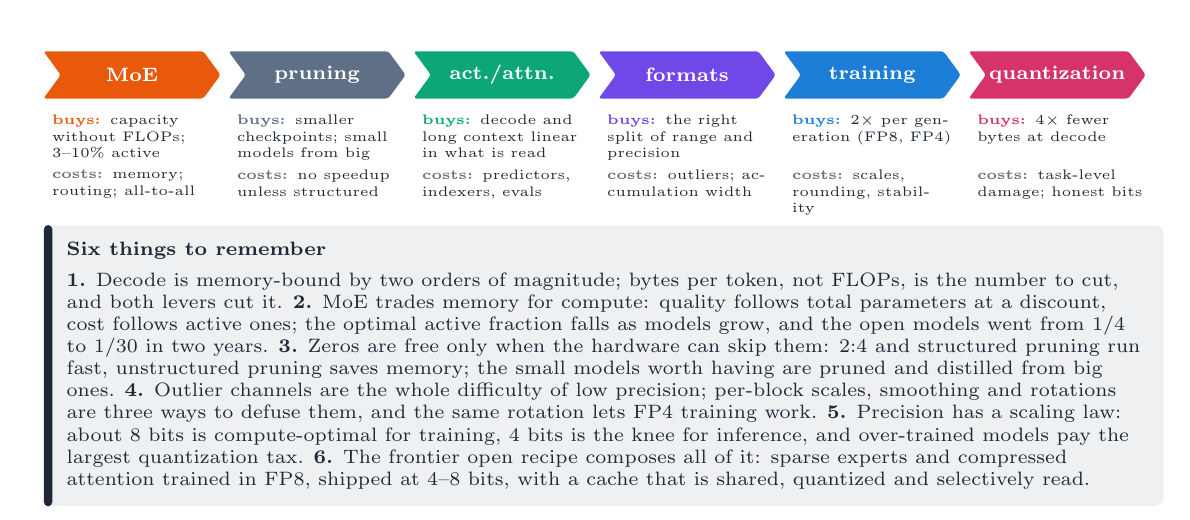
\begin{tikzpicture}
  \useasboundingbox (0,0) rectangle (14.4,5.9);
  \foreach \i/\c/\lab/\adds/\risk in {0/attn/{MoE}/{capacity without FLOPs; 3--10\% active}/{memory; routing; all-to-all},
                                      1/tok/{pruning}/{smaller checkpoints; small models from big}/{no speedup unless structured},
                                      2/emb/{act./attn.}/{decode and long context linear in what is read}/{predictors, indexers, evals},
                                      3/posc/{formats}/{the right split of range and precision}/{outliers; accumulation width},
                                      4/mlp/{training}/{2$\times$ per generation (FP8, FP4)}/{scales, rounding, stability},
                                      5/outc/{quantization}/{4$\times$ fewer bytes at decode}/{task-level damage; honest bits}}{
    \chev{0.2+\i*2.35}{5.0}{2.25}{\c}{\lab}
    \node[lab,anchor=north west,text width=2.15cm,font=\tiny,text=ink] at ({0.25+\i*2.35},4.85) {\hl{\c}{buys:} \adds};
    \node[lab,anchor=north west,text width=2.15cm,font=\tiny,text=ink] at ({0.25+\i*2.35},4.15) {\hl{muted}{costs:} \risk};}
  \bgpanels{0.2}{3.4}{13.65cm}{Six things to remember}{%
    \textbf{1.} Decode is memory-bound by two orders of magnitude; bytes per token,
    not FLOPs, is the number to cut, and both levers cut it.
    \textbf{2.} MoE trades memory for compute: quality follows total parameters
    at a discount, cost follows active ones; the optimal active fraction falls
    as models grow, and the open models went from 1/4 to 1/30 in two years.
    \textbf{3.} Zeros are free only when the hardware can skip them: 2:4 and
    structured pruning run fast, unstructured pruning saves memory; the small
    models worth having are pruned and distilled from big ones.
    \textbf{4.} Outlier channels are the whole difficulty of low precision;
    per-block scales, smoothing and rotations are three ways to defuse them,
    and the same rotation lets FP4 training work.
    \textbf{5.} Precision has a scaling law: about 8 bits is compute-optimal
    for training, 4 bits is the knee for inference, and over-trained models
    pay the largest quantization tax.
    \textbf{6.} The frontier open recipe composes all of it: sparse experts and
    compressed attention trained in FP8, shipped at 4--8 bits, with a cache
    that is shared, quantized and selectively read.}
\end{tikzpicture}
\end{frame}

% ---------------------------------------------------------------- 33
\begin{frame}{Sources}
\framesubtitle{Primary papers, checked against arXiv; $^\dagger$ marks claims taken from vendor pages, model cards, blogs or commentary.}
\begin{columns}[T]
\begin{column}{0.5\textwidth}
\fontsize{5.4}{6.4}\selectfont\color{ink}
\textbf{Mixture of experts.} Shazeer et al.\ 2017, sparsely-gated MoE, 1701.06538. Lepikhin et al.\ 2020, GShard, 2006.16668. Fedus et al.\ 2021, Switch, 2101.03961. Du et al.\ 2021, GLaM, 2112.06905. Zoph et al.\ 2022, ST-MoE, 2202.08906. Zhou et al.\ 2022, expert choice, 2202.09368. Clark et al.\ 2022, routed scaling laws, 2202.01169. Gale et al.\ 2022, MegaBlocks, 2211.15841. Jiang et al.\ 2024, Mixtral, 2401.04088. Dai et al.\ 2024, DeepSeekMoE, 2401.06066. Krajewski et al.\ 2024, fine-grained MoE laws, 2402.07871. DeepSeek-V2, 2405.04434. Wang et al.\ 2024, aux-loss-free balancing, 2408.15664. DeepSeek-V3, 2412.19437. Abnar et al.\ 2025, optimal sparsity, 2501.12370. Ludziejewski et al.\ 2025, joint MoE laws, 2502.05172. Qwen3, 2505.09388. Kimi K2, 2507.20534. gpt-oss model card, 2508.10925; Llama 4, Qwen3-Next: Meta and Qwen blogs and HF cards$^\dagger$.\\[2pt]
\textbf{Pruning and sparsity.} LeCun et al.\ 1989, OBD. Hassibi \& Stork 1993, OBS. Han et al.\ 2015, 1506.02626. Frankle \& Carbin 2019, 1803.03635. Mishra et al.\ 2021, 2:4, 2104.08378. Frantar \& Alistarh 2023, SparseGPT, 2301.00774. Sun et al.\ 2023, Wanda, 2306.11695. Frantar et al.\ 2023, sparse scaling laws, 2309.08520. Xia et al.\ 2023, Sheared LLaMA, 2310.06694. Muralidharan et al.\ 2024, Minitron, 2407.14679; Sreenivas et al.\ 2024, 2408.11796. Li et al.\ 2022, lazy neurons, 2210.06313. Mirzadeh et al.\ 2023, ReLU strikes back, 2310.04564. Liu et al.\ 2023, Deja Vu, 2310.17157. Liu et al.\ 2024, TEAL, 2408.14690. Lee et al.\ 2024, CATS, 2404.08763.\\[2pt]
\textbf{Attention.} Child et al.\ 2019, 1904.10509. Beltagy et al.\ 2020, Longformer, 2004.05150. Zaheer et al.\ 2020, BigBird, 2007.14062. Shazeer 2019, MQA, 1911.02150. Ainslie et al.\ 2023, GQA, 2305.13245. Jiang et al.\ 2023, Mistral 7B, 2310.06825. Zhang et al.\ 2023, H2O, 2306.14048. Xiao et al.\ 2023, StreamingLLM, 2309.17453. Li et al.\ 2024, SnapKV, 2404.14469. Tang et al.\ 2024, Quest, 2406.10774. Yuan et al.\ 2025, NSA, 2502.11089. Lu et al.\ 2025, MoBA, 2502.13189. DeepSeek-V3.2, 2512.02556 (V3.2-Exp, Sept 2025, GitHub$^\dagger$). DeepSeek-V4, 2606.19348; Kimi K3 model card$^\dagger$. Hsieh et al.\ 2024, RULER, 2404.06654.
\end{column}
\begin{column}{0.5\textwidth}
\fontsize{5.4}{6.4}\selectfont\color{ink}
\textbf{Formats and hardware.} Micikevicius et al.\ 2018, mixed precision, 1710.03740. Micikevicius et al.\ 2022, FP8 formats, 2209.05433. OCP Microscaling Formats spec v1.0, 2023$^\dagger$. NVIDIA, NVFP4 (developer blog, 2025)$^\dagger$. Dettmers et al.\ 2023, QLoRA/NF4, 2305.14314. GPU figures: NVIDIA A100, H100, HGX B200 datasheets; AMD MI300X, MI355X pages$^\dagger$.\\[2pt]
\textbf{Low-precision training.} NVIDIA Transformer Engine docs$^\dagger$. DeepSeek-V3, Sec.\ 3.3, 2412.19437. Tseng et al.\ 2025, MXFP4 training, 2502.20586. NVIDIA 2025, MXFP8 recipes, 2506.08027. NVIDIA 2025, NVFP4 pretraining, 2509.25149. Castro et al.\ 2025, Quartet, 2505.14669. NVIDIA, Nemotron 3 Ultra technical report, June 2026$^\dagger$; Rubin announcement, 2026$^\dagger$.\\[2pt]
\textbf{Scaling laws.} Kumar et al.\ 2024, precision, 2411.04330. Dettmers \& Zettlemoyer 2023, 4-bit, 2212.09720. Sun et al.\ 2025, FP quantization training, 2501.02423.\\[2pt]
\textbf{Quantization.} Dettmers et al.\ 2022, LLM.int8(), 2208.07339. Xiao et al.\ 2022, SmoothQuant, 2211.10438. Frantar et al.\ 2022, GPTQ, 2210.17323. Lin et al.\ 2023, AWQ, 2306.00978. Ashkboos et al.\ 2024, QuaRot, 2404.00456. Liu et al.\ 2024, SpinQuant, 2405.16406. Liu et al.\ 2024, KIVI, 2402.02750. Lin et al.\ 2024, QServe, 2405.04532. Frantar et al.\ 2024, Marlin, 2408.11743. Tseng et al.\ 2024, QuIP\#, 2402.04396. Egiazarian et al.\ 2024, AQLM, 2401.06118. Liu et al.\ 2023, LLM-QAT, 2305.17888. Ma et al.\ 2024, BitNet b1.58, 2402.17764; 2B4T, 2504.12285. Meta, Llama 3.2 quantized models (blog, Oct 2024)$^\dagger$. OpenAI, gpt-oss (blog and card, Aug 2025)$^\dagger$.\\[4pt]
\textcolor{muted}{Curves labelled \emph{illustrative} are sketches of a mechanism, not data; numbers labelled \emph{derived} were computed from published configurations (KB $=1024$ bytes, GB $=10^9$ bytes). Hardware peaks are dense unless stated and come from vendor datasheets.}
\end{column}
\end{columns}
\end{frame}
\end{document}
